%%
%% Hochschule Emden-Leer --  Abschlussarbeit
%%
%% Hauptdokument
%%
%% 23.01.09 Tschirley V.01
%% 24.08.14 Bergen V.03
%% 28.11.14 Lorenz V.04
%%
%%%%%%%%%%%%%%%%%%%%%%%%%%%%%%%%%%%%%%%%%%%%%%%%%%%%%%%%%%%%%%%%%%%%%
\documentclass[11pt, a4paper]{book}
\usepackage[hang]{footmisc}
\setlength\footnotemargin{10pt}

%% Übersetzen als Entwurf
%\usepackage[entwurf]{latexTemplate/bhtThesis}
%% Übersetzen für die Abgabe
\usepackage[abgabe]{latexTemplate/bhtThesis}	
\typeout{Master-Thesis Sascha Lorenz Hochschule Emden-Leer V0.1}
\usepackage{blindtext}   %für Blindtext, warum auch immer; ohne geht maketitle nicht: EB, 01.05.2014
\usepackage{listings}
\lstset{ 
  literate={ö}{{\"o}}1
           {ä}{{\"a}}1
           {ü}{{\"u}}1
           {Ö}{{\"O}}1
           {Ä}{{\"A}}1
           {Ü}{{\"U}}1
           {ß}{{\ss}}2
}

% Symbole
\usepackage{trsym} % http://ftp.gwdg.de/pub/ctan/fonts/trsym/trsym.pdf
\usepackage{bytefield} %http://ftp.uni-erlangen.de/mirrors/CTAN/macros/latex/contrib/bytefield/bf-example.pdf
\usepackage{bibgerm}
\usepackage{MnSymbol}
\usepackage{lmodern}
\usepackage{multibib}
\usepackage{amsmath}
\usepackage{amssymb}
\usepackage{amstext}
\usepackage{amsfonts}
\usepackage{mathrsfs}
\usepackage[onehalfspacing]{setspace}

%\usepackage[acronyms]{glossaries}
\usepackage[acronym,style=long,toc=true,numberedsection=autolabel]{glossaries} 
%\robustify{\gls}

\usepackage{booktabs}
\makeglossaries

\usepackage{tikz}
\usetikzlibrary{shapes.geometric, arrows}

\tikzstyle{startstop} = [rectangle, rounded corners, minimum width=3cm, minimum height=1cm,text centered, draw=black, fill=red!30]
\tikzstyle{io} = [trapezium, trapezium left angle=70, trapezium right angle=110, minimum width=3cm, minimum height=1cm, text centered, draw=black, fill=blue!30]
\tikzstyle{process} = [rectangle, minimum width=3cm, minimum height=1cm, text centered, draw=black, fill=orange!30]
\tikzstyle{decision} = [diamond, minimum width=3cm, minimum height=1cm, text centered, draw=black, fill=green!30]
\tikzstyle{block} = [rectangle, draw, fill=blue!20, 
    text width=8em, text centered, rounded corners, minimum height=6em]



\newcites{lit}{Literaturverzeichnis}
\newcites{int}{Internetquellen}
\usepackage{framed}

\usepackage{listings,xcolor}

\definecolor{listingBackground}{rgb}{0.97,0.97,0.97}
\definecolor{stringColor}{rgb}{0.37,0.37,0.37}
\lstset{
	basicstyle=\footnotesize\ttfamily,
	numbers=left,
	numberstyle=\tiny,
	%stepnumber=2,
	numbersep=5pt,
	tabsize=2,
	extendedchars=true,
	breaklines=true,
	keywordstyle=\color{red},
	frame=b,
	stringstyle=\color{stringColor}\ttfamily,
	showspaces=false,
	showtabs=false,
	xleftmargin=17pt,
	framexleftmargin=17pt,
	framexrightmargin=5pt,
	framexbottommargin=4pt,
	backgroundcolor=\color{listingBackground},
	showstringspaces=false
}

\usepackage{caption}
\DeclareCaptionFont{white}{\color{black}}
\DeclareCaptionFormat{listing}{\colorbox[rgb]{0.87, 0.87, 0.87}{\parbox{\textwidth}{\hspace{15pt}#1#2#3}}}
\captionsetup[lstlisting]{format=listing,labelfont=white,textfont=white,singlelinecheck=false,margin=0pt,font={bf,footnotesize}}

\usepackage[babel,german=quotes]{csquotes}


\DeclareQuoteStyle{fquotes}
  {\em}{}{\em}{}

\newcommand*{\myfquote}[1]{%
  \begingroup%
    \setquotestyle{fquotes}%
    \enquote{#1}%
  \endgroup%
}

\newif\ifmyblockquote
\newcommand*{\myblockquote}{%
\myblockquotetrue\blockquote}

\DeclareQuoteStyle[italics]{german}
[\itshape]
[\itshape]
{\quotedblbase}
{\textquotedblleft}
[0.025em]
{\quotesinglbase}
{\fixligatures\textquoteleft}
\DeclareQuoteAlias[italics]{german}{german}


\renewcommand\mkblockquote[4]{\enquote{#1#2#3}#4}

\providecommand{\e}[1]{\ensuremath{\times 10^{#1}}}

%%
%% Pfad zu den Bildern
%%
\graphicspath{
  {pictures/},
  %{einleitung/pictures},
  %{kapitel1/pictures/},
  %{kapitel2/pictures/}
}

%\usepackage{pgfplots}
%\usepgfplotslibrary{dateplot}



%%
%% Einbinden persönlicher macros 
%%
%
% Persönliche Macros
%
%

% Macros für Formeln
\newcommand{\jw}{j\omega}

% Begriffe

\newcommand{\OPV}{Operations\-ver\-stär\-ker}

\newcounter{itemlist}[chapter]
\renewcommand*{\theitemlist}{\thechapter.\arabic{itemlist}}

\newenvironment{itemlist}[2]{%
  \refstepcounter{itemlist}%  
  \hspace*{1em} \\ {Liste~\theitemlist ~-~#1:\ } \label{#2}	
  \begin{itemize}
}{%
  \end{itemize}
}

%% Message
\typeout{-----------------------------------------------------------}
\typeout{----> thesis.tex ---- Zentrales Dokument-------------------}
\typeout{-----------------------------------------------------------}

\version{1.56}
\abgabedatum{{07}. {März} {2015}}
%%
%% Titel, Autor und Betreuer
%%
\fachbereich{Technik} 
\studiengang{Medieninformatik (Master)}
\autor{Sascha P. Lorenz}
\matrnr{501 63 21}
\titel{Big Data Processing mit Apache Spark}
\untertitel{}
\betreuerFeld{
  \begin{tabular}{llr}
    
    \textbf{1. Betreuer} & Prof.~Dr.~Stefan~Edlich & Beuth Hochschule für Technik Berlin\\
    \textbf{2. Betreuer} & Prof.~Dr. Schiemann-Lillie & Hochschule Emden-Leer
  \end{tabular}
}

%%\renewcommand{\baselinestretch}{1.05} 
\renewcommand{\arraystretch}{1.3}
\pagenumbering{Alph}
\begin{document}
\pagestyle{fancy}
\newacronym{glo:mpeg}{MPEG}{Motion Pictures Expert Group}


\cleardoublepage

%%
%% Beuth Hochschule für Technik --  Abschlussarbeit
%%
%% Titelseiten und Erklärungen 
%%
%%%%%%%%%%%%%%%%%%%%%%%%%%%%%%%%%%%%%%%%%%%%%%%%%%%%%%%%%%%%%%%%%%%%%

\maketitle
\clearpage
\thispagestyle{empty}
% Rueckseite (leer)
%% 
~
\newpage

%%
%% Abstract
%%
%%%%%%%%%%%%%%%%%%%%%%%%%%%%%%%%%%%%%%%%%%%%%%%%%%%%%%%%%%%%%%%%%%%%%

%% Wird am Ende der Arbeit nochmals überarbeitet/angepasst

\section*{Kurzfassung}
Gegenstand dieser Arbeit sind die Grundlagen der Verarbeitung und Analyse großer Datenmengen (Big Data) am konkreten Beispiel von Apache Spark. Zunächst sollen verschiedene Ansätze mit Ihren Funktionsweisen sowie den Vor- und Nachteilen diskutiert werdem. Hier werden zuerst allgemeine Grundlagen zu Big Data erarbeitet. Was ist Big Data, was unterscheidet die Verarbeitung von strukturierten und unstrukturierten Daten, Relationale Datenbanken vs. noSQL, wie müssen die Quelldaten für die jeweiligen Verarbeitungen beschaffen sein, welche besonderen Herausforderungen stellen gestreamte Daten an die Verarbeitung. Besonders wird hier auf Hadoop und den Map/Reduce-Algorithmus eingegangen, um das bisher etablierte Vorgehen zu beschreiben und ein grundsätzliches Verständnis für die Domäne ``Big Data Processing'' zu schaffen. In diesem Kontext wird das gesamte Ökosystem rund um Hadoop vorgestellt. 

Nachdem eine Einführung in das Thema ``Big Data Processing'' erfolgt ist und ein entsprechend quantitativ und qualitativ brauchbarer Datensatz zur Verfügung steht, werden die Next-Generation Data-Processing Technologien betrachtet. Kernthema ist hier Apache Spark und der gesamte BDAS (Berkeley Data Analytics Stack), der von den den AMP-Labs innerhalb von Apache-Projekten um Spark herum aufgebaut wurde. Zu praktisch jeder ``offiziellen" BDAS-Implementierung existieren noch Alternativen. Besonders Apache flink wird hier als Alternative näher untersucht. Auch Applikationen, die auf dem eigentlichen Stack aufsetzen, werden näher betrachtet und entsprechenden Praxistests unterzogen (beispielsweise H2O für statistische Analysen). 

Danach wird die API von Spark und deren Möglichkeiten mit Scala, Java und Clojure näher betrachtet und durch jeweils eigene Implementierungen untersucht. 

Die Arbeit schließt mit durch verschiedene Versuchsreihen fundierte Empfehlungen für die unterschiedlichen Anforderungen im Bereich des Big-Data-Processing.



%% eof

%%
%% Abstract
%%
%%%%%%%%%%%%%%%%%%%%%%%%%%%%%%%%%%%%%%%%%%%%%%%%%%%%%%%%%%%%%%%%%%%%%


\section*{Abstract}


%% eof

%\clearpage

%\ifthenelse{\boolean{@entwurfset}}
%    {

%    }
%    {
%      ~
%      \newpage
%      \vfill
%      \section*{Aufgabenblatt -- durch Original austauschen !!!}
%      \vfill
%      \clearpage
%      ~
%      \newpage
%    }
%\vspace{10ex}
%\section*{Erklärung}
%Ich  versichere, dass  ich diese  Abschlussarbeit ohne  fremde  Hilfe selbstständig
%verfasst und  nur die  angegebenen Quellen und  Hilfsmittel benutzt  habe. Wörtlich
%oder dem  Sinn nach  aus anderen  Werken entnommene Stellen  sind unter  Angabe der
%Quellen kenntlich gemacht.
%\vspace{10ex}\\

%\hrule
%{\small{Datum}}\hfill{\small{Unterschrift}}


\pagenumbering{roman}
\setcounter{tocdepth}{1}
\tableofcontents

\frontmatter



\mainmatter

\pagenumbering{arabic}
%%%%%%%%%%%%%%%%%%%%%%%%%%%%%%%%%%%%%%%%%%%%%%%%%%%%%%%%%%%%%%%
%% Die Kapitel der Arbeit

\chapter{Einführung}
\label{chapter:einfuehrung}

\textit{Big Data} ist insbesondere in den letzten Jahren immer stärker in den verschiedensten Zusammenhängen in den allgemeinen Sprachgebrauch vorgedrungen und ist hier einem ständigen Bedeutungswandel ausgesetzt. Besonders in letzter Zeit wird dieses Thema auch verstärkt kontrovers diskutiert.  

Im ersten Kapitel soll der Begriff \textit{Big Data} jenseits von Management-Hype und Skepsis rational definiert werden. Des Weiteren werden einige grundlegende Konzepte des Umgangs mit sehr großen und unstrukturierten Datensätzen diskutiert und im Speziellen die Motivation hinter den Apache Frameworks Hadoop und Spark vorgestellt.  

Das zweite Kapitel beschäftigt sich mit dem Berkeley Data Analytics Stack (BDAS), mit dem von der UCLA Berkeley rund um Hadoop ein leistungsfähiger Infrastruktur-Stack für die Einsatzbereiche von Big Data Analytics geschaffen wurde. 

Innerhalb vom BDAS etabliert sich langsam auch eine schnellere und flexiblere Alternative zu Hadoop: Apache Spark. Im dritten Kapitel wird diese neue Kerntechnologie vorgestellt, die zugleich auch den Hauptteil dieses Wissenschaftlichen Projektes darstellt. 

Im vierten Teil dieser Ausarbeitung wird Spark in der praktischen Anwendung gezeigt inklusive Installation und ersten kleineren Beispielen sowohl direkt in Spark, als auch aus darüber liegenden Schichten aus dem Stack. 

\section{Was versteht man unter \textit{Big Data}?}
\label{section:was versteht man unter Big Data?}


Der Begriff \textit{Big Data} wurde vermutlich zum ersten Mal Ende des 20. Jahrhunderts von John R. Marshey, damals Chefwissenschaftler bei Silicon Graphics, im Rahmen einer Usenix-Konferenz öffentlich erwähnt \citeint{jt11}. Mittlerweile ziert dieser Begriff gefühlt jedes zweite Cover von IT-Zeitschriften mit Business-Fokus und auch Manager und \textit{Sales-Professionals} werten Ihre Produktpräsentationen gerne mit diesem Buzzword auf.  Aber dieser Begriff ist nicht nur positiv assoziiert. Besonders seit Bekanntwerden der Tätigkeiten des Amerikanischen Auslandsgeheimdienstes weckt die Vorstellung des Datensammelns in großen Dimensionen auch Misstrauen. 

Im Rahmen dieser Arbeit soll jedoch ausschließlich die technische Betrachtung und die exemplarische Darstellung von möglichen Anwendungsgebieten diskutiert werden.




Wie lässt sich der Begriff \textit{Big Data} abgrenzen? Es existiert keine abschließend eindeutige Definition, jedoch gibt es einige Attribute, die sich in einem Großteil der Fachliteratur etabliert haben. Der Artikel aus dem O'Reilly Radar zum Thema \citeint{dumbhill} fasst dies folgendermaßen zusammen: 

\enquote{Big data is data that exceeds the processing capacity of conventional database systems. The data is too big, moves too fast, or doesn’t fit the structures of your database architectures.}

Neben der reinen Menge spielt also offensichtlich auch die mangelnde oder fehlende Strukturierung und unter Umständen die Flüchtigkeit der Daten eine nicht unerhebliche Rolle. Dies können beispielsweise Daten aus Social-Media-Quellen sein, die aus allen möglichen verschiedenen Einzeldaten bestehen, Daten von Sensoren, die permanent überwacht werden müssen, oder Datenströme (Video, Audio, Bilder, Text), die nach einheitlichen Kriterien gefiltert werden sollen, um hier nur einige Beispiele zu nennen. Auch die temporäre Komponente ist ein Einsatzgebiet für \textit{Big Data}, und auch hier ist wieder das Beispiel der Datenströme heranzuziehen. 

Bei der Definition von \textit{Big Data} werden laut des BITKOM-Ratgebers zum Thema \textit{Big Data} \citeint{bk14} auch immer wieder die „Three Vs“ angeführt. Dies sind \textit{Volume}, also die Datenmenge, \textit{Variety}, die Datenvielfalt und \textit{Velocity}, die Geschwindigkeit der Auswertung. 

Die sinnvolle Analyse dieser Daten kann Unternehmen oder anderen Organisationen wichtige Informationen z.B. über Marktentwicklungen, bestimmte Kundenbedürfnisse, Epedemie-Ausbreitungen oder andere wichtige Sachverhalte liefern. Diese Analyse inklusive der dazu verwendeten Werkzeuge wird allgemein \textit{Big Data Analytics} genannt. 

\section{Ansätze für \textit{Big Data Analytics}}
\label{section:ansaetze für Big Data Analytics}


Die Disziplin \textit{Big Data Analytics} umfasst Methoden und Werkzeuge zur automatisierten oder interaktiven Erkennung und daraufhin auch Verwendung von bestimmten Mustern und Assoziationen. Dies sind unter anderem:

\begin{itemize}
		\item Prediction-Models zur Vorhersage bestimmter Sachverhalte
		\item statistische Verfahren, wie beispielsweise \textit{Logistic Regression} oder \textit{k-means-Algorithmen} 
		\item Optimierungs- und Filteralgorithmen 
		\item Werkzeuge zum Datamining
		\item Textanalyse
		\item Bild- und Tonanalyse
		\item Datenstromanalysen
\end{itemize}	



Nach dem BITKOM-Leitfaden \citeint{bk14} besteht die Taxonomie der Big-Data-Technologien grundsätzlich aus vier Schichten:


\begin{itemize}
		\item Daten-Haltung
		\item Daten-Zugriff 
		\item Analytische Verarbeitung
		\item Visualisierung
\end{itemize}	


Diese werden durch \textit{Daten-Integration} und \textit{Daten-Governance}, sowie Daten-Sicherheit flankiert, um den Weg von Rohdaten bis zu nutzbaren Erkenntnissen in existierende Standards einzubetten.

Zahlreiche Hersteller herkömmlicher relationaler Datenbanksysteme versuchen derzeit, ihre bestehenden Lösungen mit dem Label \textit{Big Data} zu versehen und diese so weiterhin in diesen sich verändernden Marktsegmenten zu positionieren. Wenn \textit{Big Data} jedoch jenseits der Datengröße definiert wird und auch unstrukturierte und temporäre Daten-Stacks oder –ströme zu verarbeiten oder zu analysieren sind, stoßen RDBMS \footnote{RDBMS = Relational Database Management System, also ein relationales Datenbanksystem (im Gegensatz zu Objekt- oder Graphdatenbanken).} sehr schnell an ihre Grenzen. Doch auch was die Skalierbarkeit angeht, sind relationale Datenbanken meist nicht hinreichend flexibel \citeint{ml10}. 

Für die Anforderungen an dedizierte Aufgaben im Bereich \textit{Big-Data-Analytics} sind seit einigen Jahren einige \textit{Frameworks} auf dem Markt, die in allen drei oben genannten Aspekten besser geeignet sind, als RDBMS. Der Ansatz ist hier primär, die Verarbeitung zu dezentralisieren, also auf unabhängige Knoten in einem Rechner-Cluster zu verteilen und nur Referenzen auf die Clusterknoten zentral zu verwalten.  

Es existieren mittlerweile Lösungen am Markt, die speziell diese Aufgaben für derartige Aufgaben entwickelt wurden. Hier wären unter anderem Hadoop, Spark, HPCC, GPMR, Mincmeat, Sphere, Bashreduce und R3 zu nennen. Bis auf HPCC setzen alle eben genannten Implementierungen generell oder in Teilen auf das Programmiermodell MapReduce. 

Der zweifellose De-facto-Standard in diesen Bereichen ist bereits seit einiger Zeit das Open-Source-Framework Apache Hadoop. Auf Hadoop basierend existieren etliche Derivate. Unter anderem sind hier Cloudera, Amazon Elastic MapReduce, Apache BigTop, Datameer, Apache Mahout, MapR und IBM PureData System zu nennen. 



	





\section{Motivation für Apache Hadoop/Spark}
\label{section:motivation für Apache Hadoop/Spark}

Anfang des 21. Jahrhunderts wurde das Bedürfnis für Möglichkeiten, sehr große Datenmengen effizient verarbeiten zu können, stetig größer. Nicht zuletzt durch die zu dieser Zeit exponentiell steigende Menge von Inhalten im World Wide Web und deren Indexierung durch Suchmaschinen wie Google. Davon motiviert wurde 2002 das Projekt \textit{Nutch} mit dem Ziel gestartet, ein geeignetes \textit{Such- und Crawlersystem} frei verfügbar zu machen. Die ersten Versuche skalierten sehr schlecht, bis Google 2003 die Funktionsweise ihres verteilten Dateisystem GFS (Google File System) veröffentlichte. Somit konnten die sehr großen Dateien, die durch die Indexierung entstanden, effizient auf verschiedene Knoten verteilt gespeichert werden und die Verwaltung dieser Knoten und Dateien aus dem eigentlichen Indexierungs- und Suchprozess ausgelagert werden. 

Im Jahre 2004 publizierte Google den \textit{MapReduce-Algorithmus}, der unter anderem die Indexie-rungs- und Analysefunktionen parallelisieren, delegieren und sinnvoll bündeln kann. In Nutch wurden daraufhin sämtliche wichtige Algorithmen auf MapReduce umgestellt, nachdem zuvor auch GFS unter dem Namen NDFS (Nutch Distributed File System) integriert wurde. Die möglichen Anwendungsgebiete von Nutch waren damit auch weit über das reine Suchen und Indexieren von Webseiten hinaus gewachsen. 2006 wurde aus Nutch ein Unterprojekt mit dem Namen Hadoop ausgegliedert, das im Jahre 2008 zum \textit{Apache Top-Level-Projec}t ernannt wurde. Zu dieser Zeit nutzten bereits Firmen wie Yahoo!, Facebook oder die New York Times Hadoop. Ein exemplarischer Anwendungsfall bei der NY Times war, mit Hilfe der Hadoop-basierten EC2-Cloud von Amazon ca. vier Terabyte gescannter Archivdateien in PDF-Dateien umzuwandeln und dies in weniger als 24 Stunden auf 100 Knoten. Auch beim Sortieren von sehr großen Datenmengen stellten Hadoop-basierte Systeme nach und nach sämtliche Rekorde ein \citelit{tw13}. 

Hadoop und Hadoop-basierte System gelten mittlerweile als Industriestandard für Big-Data-Analytics-Anwendungen. Jedoch ist Hadoop nicht für alle Anwendungsgebiete gleichermaßen geeignet. Aufgrund der Charakterisierung der Paradigmen für Big Data Analytics im Paper „Frontiers in Massive Data Analysis“ der National Academic Press \citelit{nrc13}, lassen sich die Einsatzgebiete und Schwächen für Hadoop ermitteln \citelit{va14}.

So lassen sich mit Hadoop einfachere statistische Aufgabenstellungen sehr gut umsetzen. Dazu gehören Mittelwert, Median, Varianz und allgemein abzählende sowie ordnende Statistikaufgaben. Dies sind in der Regel Anwendungen mit einer Laufzeitkomplexität von O(n) für n Betrachtungswerte. Sie sind meist auch sehr gut parallelisierbar und somit sehr gut für Hadoop geeignet.    



Für linear-algebraische Berechnungen (lineare Regression, Eigenwertproblem, Hauptkomponentenanalyse), generalisierte n-Körper-Probleme (mit einer Komplexität 
von O(n²) oder O(n³)), Graphentheorie, Optimierungsprobleme (Verlust-, Kosten- oder Energiefunktionen, sowie  Inte-grations- und Ausrichtungsfunktionen ist \textit{Hadoop} nur in jeweils einfacher Problemausprägung einsetzbar. Auch für Interaktive Abfragen ist \textit{Hadoop} nur bedingt geeignet, da es ursprünglich für die \textit{Batch-Verarbeitung} entwickelt wurde.

Aus diesem Grund wurde am \textit{AMPLab} der University of California in Berkeley nach Alternativen geforscht, die auch für komplexe linear-algebraische Probleme, generalisierte n-Körper-Probleme und diverse Optimierungsprobleme geeignet sind. Das Ergebnis ist \textit{Spark}, mittlerweile \textit{Apache Top-Level-Projekt} und dazu geeignet, die Nachfolge von Hadoop als \textit{Big-Data-Analytics-Framework} anzutreten. 

\section{Ziel und Aufbau dieser Arbeit}
\label{section:ziel dieser Arbeit}

Die vorliegende Arbeit beschäftigt sich mit \textit{Apache Spark} und dem dazugehörigen Ökosystem bestehend aus Schichten mit verschiedenen Bibliotheken, dem \textit{Berkeley Data Anaytics Stack (BDAS)}. Auf dem Markt befindet sich bislang noch verhältnismäßig wenig Literatur zu diesem Thema und wenn, dann werden zumeist Teilaspekte für bestimmte Anwendungsbereiche gekapselt betrachtet. Diese Arbeit soll, nachdem einige Grundlagen zum Thema \textit{Big Data Analytics} im Allgemeinen diskutiert werden, zunächst einen ganzheitlichen Überblick über den BDAS bieten. Hier werden die einzelnen Schichten des Stacks kurz beschrieben und gegebenenfalls Alternativlösungen zu den jeweiligen Implementierungen vorgestellt. 

Insbesondere werden in den darauffolgenden Kapiteln die Statistik- und Vorhersagebibliotheken \textit{MLLib} betrachtet, in einigen Punkten mit der Alternativbibliothek \textit{H2O} verglichen und die Kernimplementierung von Spark mit dem neueren Framework \textit{Apache Flink} \footnote{Entwickelt von der Technischen Universität Berlin zunächst unter dem Namen \textit{Stratosphere} und mittlerweile (Stand Ende 2014) \textit{Apache Incubator} Projekt} verglichen. Auch die übrigen Elemente des BDAS wie das Caching-Frameworks Tachyon, sowie die Streaming-Bibliothek Spark Streaming und die Graphenanwendung GraphX werden vorgestellt. 

Im letzten Teil dieser Arbeit werden jeweils praktische Anwendungsbeispiele gezeigt und im Zuge dessen die APIs \footnote{API = Application Programming Interface. Schnittstelle, die von einem Softwaresystem für die Einbindung in andere Softwwaresysteme zur Verfügung gestellt wird.}von Spark und MLlib insbesondere vorgestellt.   



\chapter{Allgemeine Grundlagen }
\label{chapter:allgemeine Grundlagen}


Das nachfolgende Kapitel behandelt die Grundlagen, die für ein Verständnis der Anwendungsbereiche von Apache Spark, dem Berkeley Data Analytics Stack und im Allgemeinen des Themenkomplexes Big Data Analytics und insbesondere für Machine-Learning-Anwendungen nötig sind. Im ersten Unterkapitel werden die grundsätzlichen Eigenschaften eines verteilten Systems beschrieben um die Basis für die in der Arbeit beschriebenen Besonderheiten von Verarbeitungen im Clusterbetrieb zu legen. Hier wird ein exemplarischer Clusteraufbau skizziert, Probleme mit Concurrency und Netzwerkverkehr beschrieben und welche Möglichkeiten es hier gibt.  Im darauf folgenden Unterkapitel werden grundlegende Problemstellungen und Technologien beschrieben, die im Rahmen von Big Data Analytics im Allgemeinen vorkommen. Unter anderem werden hier Grundlagen und Begriffe aus den Themengebieten Anwendungen von Big Data Analytics, Machine Learning, Klassifikation, Vorhersagen, statistische Analysen, Graph-Suchen und Streaming-Frameworks in erklärt. Besonders die Algorithmen, die in den Machine-Learning-Implementierungen MLibs und H20 zum Einsatz kommen, werden hier detaillierter vorgestellt. In einer Zusammenfassung werde diese Grundlagen nochmals auf einen Blick dargestellt. 
 

\section{Cluster Computing}
\label{section:cluster computing}

Die Nachfrage nach immer mehr Rechenleistung hat in dein letzten Jahren dazu geführt, dass verstärkt Rechnercluster eingesetzt werden. Alternativ gibt es den Ansatz, Mainframes\footnote{Unter Mainframe wird hier ein sehr leistungsfähiges Rechnersystem verstanden, das einen oder  beliebig viele Prozessoren in einer physischen Einheit, also einem logischen Mainboard verbindet. } mit immer mehr Rechenleistung auszustatten, diese jedoch ausdrücklich autonom zu betreiben\footnote{In diesem Kontext kann durchaus ein Failover-Cluster vorhanden sein, also eine Mainframe wird zur Ausfallsicherheit repliziert. Dies wird an dieser Stelle jedoch nicht als Cluster im eigentlichen Sinn bezeichnet.}. Je nach Aufgabenspektrum ist die eine oder andere Infrastruktur besser geeignet. In der Regel wird ein geclustertes System dort eingesetzt, wo hohe Verfügbarkeit oder gut parallelisierbare Aufgaben vorherrschen. Bei netzwerkintensiven Aufgaben, wie z.B. als Webserver oder Datenbanksystem sollten in der Regel besser Installationen auf einem autonomen System eingesetzt werden \citelit{clus1}.   

Ein Rechner-Cluster besteht in der Regel aus mehr oder weniger eng miteinander verbundenen Computern, wobei hier im Gegensatz zu Mainframes jeder Rechner über eigene Ressourcen wie Hauptspeicher, Massenspeicher, etc. verfügt. Ein Cluster, bzw. ein Verteiltes System ist nach Andrew S. Tanenbaum \citelit{tan1} folgendermaßen definert: 

\enquote{A distributed system is a collection of independent computers that appears to its users as a single coherent system.}

Bei der Verwendung eines Clusters sind einige Besonderheiten zu beachten, die bei der Ausführung auf gewöhnlichen Systemen nicht ins Gewicht fallen \citelit{tan1}. Unter Anderem sind die Tasks so gestalten, dass möglichst wenig Wartezeit durch Abhängigkeiten entsteht und diese möglichst autonom verarbeitet werden können. Außerdem muss beachtet werden, dass die einzelnen Knoten eines Clusters über Messaging-Mechanismen miteinander kommunizieren und dies insbesondere hohe Anforderungen an die Netzwerkinfrastruktur stellt. Eine typische Clustertopologie besteht aus mehreren Worker-Knoten und einem Masterknoten. Der Masterknoten deligiert die Tasks an die einzelnen Worker-Knoten und stellt das gesamte Cluster nach außen hin als ein geschlossenes System dar. Sämtliche Kommunikation mit dem Cluster findet grundsätzlich nur über den Masterknoten statt.


 
\section{Anwendungen für Big Data Analytics}
\label{section:anwendungen für big data analytics}

Im folgenden Unterkapitel werden exemplarisch einige Anwendungsfälle für \textit{Big Data Analytics} (auch \textit{Data Mining}) dargestellt, um zu klären, für welche Einsatzbereiche \textit{Frameworks} wie \textit{Apache Spark} und die darauf aufbauenden Bibliotheken in der Praxis benötigt werden.  

Laut Arvind Sathi \citelit{bda1} zeichnet sich \textit{Big Data} unter Anderem durch ein mögliches Vorkommen von unstrukturierten Daten aus. Die Autoren Chakraborty und Pagolu gehen in ihrem Artikel \citeint{ckb11} davon aus, dass mittlerweile mehr als 80\% der gesamten Daten im digitalen Raum in unstrukturierter Form vorliegen. In der Vergangenheit mussten für Analysetätigkeiten in aller Regel strukturierte Datensätze vorliegen. Grundsätzlich ist es mit den gängigen \textit{Data Analytics Frameworks} nach wie vor möglich, beispielsweise quantitative Analysen auf strukturierten Datensätzen durchzuführen oder unstrukturierte Datensätze nachträglich zu strukturieren, um wiederum quantitative Analysen darauf anwenden zu können.

Das Potential dieser \textit{Frameworks} zeigt sich jedoch dann in vollem Umfang, wenn auf unstrukturierten Daten diverse Analysemethoden oder Verarbeitungen angewendet werden. In jüngerer Vergangenheit ist das Aufkommen unstrukturierter Daten, wie bereits erwähnt, erheblich gestiegen. Dies wird nicht zuletzt durch die massive Verbreitung von Sensoren aller Art verursacht. Dies können \textit{Logdaten}, Bewegungsdaten, Sensorwerte zur Überwachung von technischen Einrichtungen, Messwerte aus Wetterstationen und unzähligen weiteren Quellen sein. Auch viele Internetanwendungen, besonders wenn es sich um laufende Datenströme handelt, verursachen erhebliche Datenmengen, die entweder \textit{persistiert} oder sogar zur Laufzeit analysiert werden können.  

\textit{Data Mining}\footnote{Ein Großteil der Literatur verwendet die Begriffe \textit{Big Data Analytics }und \textit{Data Mining} synonym. \textit{Machine Learning} wird jedoch von \textit{Data Mining} abgegrenzt, da letzteres eine explorative Datenanalyse darstellt.} ist laut \citelit{cl14} ein analytischer Prozess mit dem Zweck, große Datenmengen nach konsistenten Mustern oder systematischen Beziehungen zu untersuchen. Die Ergebnisse werden in der Regel validiert, in dem gefundene Muster oder Ähnlichkeiten auf einer Teilmenge der ermittelten Daten angewendet werden. Ein weiteres Ziel von \textit{Data-Mining-Prozessen} sind Vorhersagen von Ereignissen mittels geeigneter Algorithmen (Vergleich \citelit{cl14} und \ref{section:machine learning}). 

Der Prozess des Data Mining setzt sich nach \citelit{mit96} im Wesentlichen aus einem oder mehreren der folgenden Aufgabenbereiche zusammen:

\begin{itemize}
		\item \textbf{Klassenbeschreibung:} Eine knappe Beschreibung der Charakterisierung der Datensätze, um sie eindeutig von anderen Daten unterscheiden zu können. 
		\item \textbf{Assoziation:} Die Untersuchung der Daten nach assoziativen Verbindungen oder Korrelationen zwischen einzelnen Daten oder Datengruppen.   
		\item \textbf{Klassifizierung:} Hier wird ein definierter Satz von Trainingsdaten\footnote{Trainingsdaten können beispielsweise Daten sein, die bereits im Vorfeld manuell klassifiziert wurden, deren Klassenzugehörigkeit also bekannt ist.} analysiert und anhand deren Beschaffenheit ein Modell generiert. Durch die Klassifizierung werden Entscheidungsbäume (Vergleich Kapitel \ref{section:machine learning}) oder Klassifizierungsregeln generiert, die schließlich für die Klassifizierung folgender Daten verwendet werden \citelit{pdl97}. 
		\item \textbf{Vorhersage:} Die Vorhersage bezieht sich auf mögliche Werte von nicht-vorhandenen Daten oder Datenspektren, die wiederum durch \textit{Approximation} einer Funktion mittels Beispielen durchgeführt wird \citelit{cl14}. Dies sind ebenfalls Trainingsdaten, die aus Datensätzen mit den dazugehörigen berechneten Funktionswerten bestehen. 
		\item \textbf{Cluster-Analyse:} Diese dient dazu, \textit{Cluster} innerhalb von Datensätzen zu ermitteln. Dies sind Daten, die definierte Ähnlichkeiten zueinander aufweisen. 
		\item \textbf{Zeitreihenanalysen:} Hier werden in der Regel große Mengen an Zeitreihendaten analysiert, um nach Ähnlichkeiten oder Mustern innerhalb der Daten zu suchen.  
		
\end{itemize}	

\newpage


\section{Machine Learning}
\label{section:machine learning}

\enquote{Learning denotes changes in the system that are adaptive in the sense that they enable the system to do the same task (or tasks drawn from a population of similar tasks) more effectively the next time.} \citelit{sim83}

Unter \textit{Machine Learning} wird ein interdisziplinärer Teilbereich der Informatik und der Statistik verstanden. Ziel ist die Erstellung von Algorithmen, die in der Lage sind, selbstständig auf Grund von Daten iterativ zu lernen gemäß der oben zitierten Definition. Um dies zu erreichen, erstellen diese Algorithmen basierend auf den jeweiligen Eingabedaten Modelle, die Entscheidungen oder Vorhersagen treffen können \citelit{isl13}. In den Abbildungen \ref{fig:MLP1} und \ref{fig:MLP2} wird dies veranschaulicht. 


\begin{figure}[htb!]
\centering
\begin{tikzpicture}[node distance=2cm]
\tikzstyle{line} = [draw, -latex']

\node (start) [startstop] {Training Data};
\node (pro2b) [block, right of=start, xshift=2cm] {\textbf{Pre-Processing} \\-Normalization \\ -Dimension Reduction};
\node (pro3b) [block, right of=pro2b, xshift=2cm] {\textbf{Learning} \\-Supervised \\ -Unsupervised};
\node (pro4b) [block, right of=pro3b, xshift=2cm] {\textbf{Error Analysis}\\ -Precision/Recall \\ -Overfitting};
\node (pro5b) [process, below of=start] {Model};

\path [line] (start) |- (pro2b);
\path [line] (pro2b) |- (pro3b);
\path [line] (pro3b) |- (pro4b);
\path [line] (pro4b) |- (pro5b);


\end{tikzpicture}
\caption{Der Machine-Learning-Prozess: Phase 1 - Lernphase}
\label{fig:MLP1}
\end{figure}


\begin{figure}[htb!]
\centering

\begin{tikzpicture}[node distance=2cm]
\tikzstyle{line} = [draw, -latex']

\node (pro5b) [process] {Model};
\node (pro6b) [startstop, below of=pro5b] {Data};
\node (pro7b) [block, right of=pro5b, xshift=2cm, yshift=-1cm] {\textbf{Prediction}};
\node (pro8b) [startstop, right of=pro7b, xshift=2cm] {Predicted Data};

\path [line] (pro5b) |- (pro7b);
\path [line] (pro6b) |- (pro7b);
\path [line] (pro7b) |- (pro8b);

\end{tikzpicture}
\caption{Der Machine-Learning-Prozess: Phase 2 - Prediction-Phase (Vorhersage)}
\label{fig:MLP2}
\end{figure}

Das erste Diagramm \ref{fig:MLP1} zeigt den Lernprozess. Zunächst werden definierte Trainingsdaten einem \textit{Pre-Processing}\footnote{Das Pre-Processing kann aus \textit{Normalisierung, Dimensionsreduktion, Bildverarbeitung} oder anderen Vorarbeiten bestehen.} zugeführt (Vergleich Unterkapitel \ref{section:klassifikationsalgorithmen}). 

Danach folgt der eigentliche Lernprozess, der mit oder ohne \textit{Überwachung}\footnote{Beim überwachten Lernen (Supervised Learning) liegen der Analyse vorher angelegte Trainingsdaten zugrunde, das unüberwachte Lernen (Unsupervised Learning) erzeugt vorher gänzlich unbekannte Modelle aus gefundenen Mustern \citeint{ul04}}, als \textit{Minimalisierungsfunktion} oder mit anderen Lernalgorithmen durchgeführt wird (Vergleich Unterpunkte Clusterverfahren und Klassifikationsalgorithmen). Der Lernprozess kann entweder mit einem bestimmten Lernalogrithmus durchgeführt werden, oder mit sogenannten \textit{Ensemble-Learning-Methods}. Dies ist die Zusammenfassung von unterschiedlichen Lernalgorithmen zu einem Lernprozess, um die Vorhersageleistung zu steigern. Nach dem Lernprozess werden das erzeugte Modell einem Validierungsprozess zugeführt. Dies können \textit{Precision/Recall}\footnote{\textit{Precision:} Wie viele der ausgewählten Datensätze sind relevant. \textit{Recall:} Wieviele relevante Datensätze wurden ausgewählt. }, \textit{Overfitting}\footnote{\textit{Overfitting} bezeichnet einen Zustand, in dem bekannte Daten (Trainingsdaten) von einem Algorithmus generell akkurater erkannt werden, als Daten, die von dem Algorithmus erkannt werden sollen (Predicitions).}, oder andere Validierungsfunktionen sein. Am Ende der Prozesse entsteht ein Modell, das für verschiedenste Aufgaben eingesetzt werden kann. 

In Abbildung \ref{fig:MLP2} wird das erzeugte Modell zusammen mit produktiven Daten genutzt, um mittels geeigneter Vorhersagealgorithmen (Vergleich Unterkapitel \ref{section:klassifikationsalgorithmen}) bisher noch nicht vorhandene Datensätze erzeugen zu können.  

Die Hauptanwendungsgebiete für \textit{Machine Learning} sind sämtliche Bereiche, in denen eine Anwendung von strikten, regelbasierten Algorithmen nicht in Frage kommt \citelit{pdl97}. Beispiele für diese Bereiche sind laut \citelit{pml06} Suchmaschinen, Sprach- und Musikerkennung, Handschriftenerkennung, Spamfilter, Umgebungserkennungen und viele mehr. 



\subsection{Klassifizierung von Daten}
\label{section:klassifizierung von daten}


Im Gegensatz zu herkömmlichen \textit{Business-Intelligence-Anwendungen}\footnote{Laut \citelit{bi12} versteht man unter \textit{Business Intelligence (BI)} die Sammlung, Auswertung und Darstellung von Daten anhand definierter Prozesse.} zeichnen sich Big-Data-Anwendungen in erster Linie durch Unterschiede in der Herangehensweise und in der Formulierung der primären Fragestellungen aus. In der Vergangenheit wurden zu Beginn einer Analyse zunächst Problemstellungen formuliert und aufgrund dessen Prozesse und vor allen Dingen die zu sammelnden Daten definiert \citelit{bi12}. Mit der steigenden Etablierung von Big-Data-Anwendungen hat sich dieser Ansatz gewandelt. Hier werden zunächst sämtliche anfallenden Daten gespeichert. Auf diese Datensätze, deren Größe in relativ kurzer Zeit massiv anwachsen kann, werden erweiterte Analyseprozesse\footnote{Unter dem Begriff \textit{Advanced Analytics} sind verschiedene Werkzeugtypen aus der vorhersagenden Analyse (\textit{Predictive Analytics}), aus dem Data Mining, aus der Statistik, der Künstlichen Intelligenz, der Sprachverarbeitung und weiteren Disziplinen zusammengefasst \citelit{tdwi11}.} angewendet, die unter anderem auch Vorhersagen erlauben \citelit{tdwi11}. 
So liegen also bei Big-Data-Analytics große Datenmengen vor, ohne dass das Ziel der Analyse im Vorfeld bekannt ist. 

\subsubsection{Clusterverfahren}
\label{section:clusterverfahren}

Nun gibt es verschiedene Herangehensweisen, wie sich relevante Fragestellungen aus den vorliegenden Daten ableiten lassen. Ein sinnvoller Ansatz besteht darin, sogenannte Cluster innerhalb der Daten zu ermitteln, also ähnliche Datensätze zu entsprechenden Gruppen zusammenzufassen. Aus diesen Gruppen werden Klassen gebildet, in dem ihnen aussagekräftige Namen zugeordnet werden\citelit{cl14}. Cluster werden beispielsweise benötigt, um Kunden nach bestimmten Interessen zu gruppieren, um Zeichen auf Ähnlichkeiten für die automatischen Zeichenerkennung zu untersuchen, oder Bilder auf vergleichbare Bildpunktanordnungen oder Farbspektren, also generell überall, wo nach Ähnlichkeiten gesucht wird. 

Ein Cluster zeichnet sich dadurch aus, dass die Objekte innerhalb eines Clusters möglichst ähnlich sind, die Cluster untereinander jedoch möglichst unähnliche Inhalte besitzen. Um Ähnlichkeiten zwischen Datensätzen oder Clustern feststellen zu können, bedarf es einer Distanzfunktion, zur Ermittlung und Sicherstellung der Clustergüte einer Qualitätsfunktion (Vergleich \citelit{cl14}). 

Laut \citelit{cl14} sind für Distanz- und Qualitätsfunktionen folgende Annahmen zu treffen:  


\begin{framed}
\begin{flalign*}
&\textbf{Vorbedingungen}& \\
&X \text { (Instanzenraum) }&  \\
&E \subseteq X \text{ (Instanzenmenge) }& \\
&X\times X \to \mathbb{R}^+ \text{ (Abstandsfunktion) }&  \\
&2^{2^x} \to \mathbb{R} \text{ (Qualitätsfunktion) }& 
\end{flalign*}

Gesucht wird eine Clustermenge \(C = \{C_1,...,C_k\}\) \text{mit folgenden Eigenschaften:} \\

\(C_i \subseteq E\) \\
\(quality(C) \to max\) \\
\(C_i \cap C_j = \emptyset\) \\
\(C_1 \cup...\cup C_k = E\) \\



Die Abstandsfunktion \(dist\), die gegebene Objekte so in Teilmengen zerlegt, dass der Abstand der Objekte innerhalb einer Teilmenge (Cluster) kleiner ist, als der Abstand zu Objekten anderer Teilmengen: \\

\(\forall C_i, C_j \in C(i \neq j) : \forall x_k, x_l \in C_i, x_m \in C_j : dist(x_k, x_l) < dist(x_k, x_m)\)\\

Die Qualitätsfunktion \(quality\) beschreibt die Qualität des Clusterings basierend auf der Abstandsfunktion \(dist\): \\

\({quality}(C = \{C_1 \subseteq E,...,C_k \subseteq E\}) \to \mathbb{R}\) \\ 
\end{framed}

\newpage

Exemplarisch werden im Folgenden einige Distanzfunktionen dargestellt, die für die Clusteranalyse wichtig sind (Vergleich \citelit{uma14},  \citelit{bro98}):

\begin{itemize}
\item \textbf{Hamming-Distanz:} Hier werden die Vektorelemente der Position \(i\) zweier Vektoren miteinander verglichen. Wenn sich diese unterscheiden, wird die Distanz auf den Wert 1 gesetzt, bei gleichen Werten 0. Nachdem alle Elemente der Vektoren miteinander verglichen wurden, werden diese summiert. Ein Vorteil der Hamming-Distanz ist, dass sich Abstände zwischen metrischen, ordinalen und sogar nominalen Daten berechnen lassen. Der Nachteil dieser Distanzfunktion ist, dass Abstandsverhältnisse nicht erkannt werden, also ist beispielsweise der Abstand zwischen 2 und 3 für diese Funktion gleichwertig zum Abstand von 2000 zu 2100.

\(dist_H(x,y) = count_i(x_i \neq y_i) \)

\item \textbf{Manhattan-Distanz:} Diese Distanzfunktion hat ihren Namen aufgrund der blockweisen Anordnung der Straßenzüge in Manhattan. Distanzen werden, wie auf einem Schachbrett, durch vertikale und horizontale Bewegungen und Richtungsänderungen beschrieben. Um die Ergebnisse der verschiedenen Distanzfunktionen untereinander vergleichbar zu machen, wird der Betrag der Distanzwerte verwendet. Die Manhattan-Distanz ist nur auf metrische Daten anwendbar. Diese Distanzfunktion ist auch unter dem Namen \textit{Block-Distanz} bekannt.   

\(dist_M(x,y) = \sum_{i} \mid x_i - y_i \mid \)


\item \textbf{Euklidische Distanz:} Hier wird der direkte Abstand zwischen zwei Vektoren beschrieben, also zweier Punkte im n-dimensionalen Raum. Diese Funktion lässt sich nur auf metrische Daten anwenden. Auch hier wird durch Quadrieren und der Quadratwurzel der Differenzen eine Normalisierung erreicht, die die Distanzwerte vergleichbar macht. 

\(dist_E(x,y) = \sqrt{\sum_{i}(x_i - y_i)^2} \)

\item \textbf{Tschebyscheff-Distanz:}  Auch hier wird der Abstand zwischen zwei Punkten im n-dimensionalen Raum betrachtet. Im Unterschied zu den beiden vorhergehenden Verfahren wird hier jedoch der größtmögliche absolute Abstand zwischen allen Attributen ermittelt. Deshalb wird diese Distanzfunktion auch als \textit{Maximum-Distanz}  bezeichnet. 

\(dist_T(x,y) = max_i(\mid x_i - y_i \mid) \)

\item \textbf{Minkowski-Distanz:}  Diese Distanz-Funktion ist ähnlich zur Euklidischen Distanz. Allerdings entspricht hier der Abstand der \(n\)-ten Wurzel der Summe der  \(n\)-ten Potenzen der Differenzen. Auch diese Funktion lässt sich nur auf metrische Daten anwenden.

\(dist_K(x,y) = \sqrt[n]{\sum_{i}(x_i - y_i)^n} \)

\end{itemize}

Darüber hinaus existieren noch zahlreiche weitere Distanzfunktionen, die je nach Einsatzzweck besser oder schlechter geeignet sein können, als die dargestellten. 


\newpage


Die Clusteranalyse zählt zu den \textit{unüberwachten Lernalgorithmen (Unsupervised Learning)}. Zoubin Ghahramani beschreibt dies in seinem Artikel \textit{Unsupervised Learning} \citeint{ul04} wie folgt: 

\enquote{[...]in unsupervised learning the machine simply receives inputs x1, x2,..., but obtains neither supervised target outputs, nor rewards from its environment. It may seem somewhat mysterious to imagine what the machine could possibly learn given that it doesn’t get any feedback from its environment. However, it is possible to develop of formal framework for unsupervised learning based on the notion that the machine’s goal is to build representations of the input that can be used for decision making, predicting future inputs, efficiently communicating the inputs to another machine, etc. In a sense, unsupervised learning can be thought of as finding patterns in the data above and beyond what would be considered pure unstructured noise.}

Prinzipiell wird zwischen vier verschiedenen Clusterarten unterschieden \citelit{cl14}: 

\begin{itemize}
		\item \textbf{Partitionierendes Clustering:} Eine Menge von Datenobjekten wird in k Cluster, die um einen Medoid\footnote{Medoide sind Stellvertreterobjekte eines Clusters, deren durchschnittliche Ähnlichkeit zu allen Datenobjekten des Clusters maximal ist. Ein Medoid ist immer ein Datensatz aus dem Cluster.} oder einen Centroid\footnote{Centroide sind Vektoren der Mittelwerte der Attribute aus den Datenobjekten. Im zweidimensionalen Raum entspricht dies der Mittelwerte der x- und y-Koordinaten aller Datenobjekte.} gebildet werden, zerlegt (Vergleich \citeint{km11}). 
		\item \textbf{Hierarchisches Clustering:} Hier werden die Cluster hierarchisch aufgebaut, indem jeweils die Cluster mit der größten Ähnlichkeit, also mit der geringsten Distanz, miteinander vereinigt werden. Aus diesen vereinigten Clustern können in der Hierarchie übergeordnete Ebenen entstehen. Beim \textit{Agglomerativen Clustering} wird mit den einzelnen Datenobjekten selbst begonnen, in dem jedes Cluster aus genau einem Datenobjekt besteht. Die jeweils ähnlichsten Cluster werden vereinigt und somit zu einer neuen Hierarchieebene. Dies geschieht so lange, bis in der obersten Ebene ein Cluster mit allen Datenobjekten entstanden ist. Beim \textit{Divisiven Clustering} wird die Hierarchie in umgekehrter Reihenfolge aufgebaut, also zunächst werden alle Datenobjekte zu einem großen Cluster zusammengenommen und dieser dann iterativ anhand der  Ähnlichkeiten der Datenobjekte untereinander geteilt.  
		\item \textbf{Dichtebasiertes Clustering:} Die Cluster werden so gebildet, dass in der Umgebung eines Datenobjektes innerhalb eines Clusters möglichst viele weitere Datenobjekte liegen, die Dichte also besonders hoch ist. Die geforderte Dichte wird über Schwellenwerte definiert. 
		\item \textbf{Clustering mit Neuronalen Netzen:} Auch über neuronale Netze können Cluster gebildet werden. Die Netze werden in diesem Fall nicht überwacht trainiert (Vergleich Einleitung Kapitel \ref{section:machine learning}) und nutzen das Verfahren des \textit{Wettbewerbslernens} (Vergleich \citelit{cl14}, beispielsweise \textit{Vonoroi-Mengen}). Das Neuron, welches dem Eingabewert (dem Datenobjekt) am ähnlichsten ist, ist im jeweiligen Wettbewerb im Vorteil. 
\end{itemize}	

\newpage

Zu den Cluster-Verfahren zählen laut \citelit{ams03} und \citelit{cl14} unter Anderem folgende Algorithmen:

\begin{itemize}
		\item \textbf{klassischer k-Means-Algorithmus (partitionierendes Verfahren):} Wie bei allen partitionierenden Verfahren werden zunächst die Clusterzahl \textit{k} und je Cluster ein Zentrum definiert. Die Zentrumsdefinition, und somit die Clusterbildung findet zufällig statt. Die Repräsentation des Clusters erfolgt durch den Centroid, also den Schwerpunkt. Eine Fehlerfunktion wird iterativ minimiert, indem die euklidischen quadrierten Abstände der Inhaltsobjekte zu den Centroiden hin verschoben werden. Nach jedem Iterationsschritt werden durch Mittelwertbildung die Centroiden neu definiert. Dieses Verfahren wird so lange iterativ durchgeführt, bis kein Datenobjekt mehr sein Cluster wechselt. Der k-Means-Algorithmus setzt metrische Werte\footnote{\textit{Metrisch}: Merkmal, das aus einer Zahl besteht und Dimension, sowie Nullpunkt besitzt (z.B. Geschwindigkeit, Einkommen, Alter), \textit{ordinal}: Merkmal mit natürlicher Ordnung (z.B. Schulnoten sehr gut, gut, befriedigend,...), \textit{nominal}: Merkmal ohne natürliche Ordnung (z.B. Geschlecht, Name)} voraus. Die Umwandlung von ordinalen Daten in metrische ist meist einfach umzusetzen, nominale Daten können mittels \textit{Binarisierung} in numerische Werte gewandelt werden. Alternativ kann auch ein modifiziertes \textit{k-Means-Verfahren} eingesetzt werden (Vergleich \citelit{cl14}, Kapitel 8).
		\item \textbf{k-Medoid-Verfahren (partitionierende Verfahren):} Im Unterschied zum k-Means-Algorithmus wird hier nicht der Centroid, sondern der Medoid als Stellvertreter für ein Cluster definiert. Ein Medoid muss immer ein Element der Datenobjekte sein. Durch Vertauschung wird nun iterativ nach qualitativ hochwertigeren Medoiden gesucht, also solchen, deren mittlere Distanz zu den anderen Datenobjekten im Cluster geringer ist. Dies wird so lange durchgeführt, bis kein Tausch der Medoiden mehr stattfindet, also jedes Cluster seinen qualitativ hochwertigsten Medoid besitzt. Die beiden wichtigsten k-Mediod-Verfahren sind PAM (Partitoning Around Medoids) und CLARANS (Clustering Large Applications based on RANdomized Search) (Vergleich \citelit{cl02}). Bei PAM wird jeweils nach dem besten neuen Mediod mit Hilfe einer Qualitätsverbesserung durch graphische Repräsentation der Datenobjektverteilung und -häufigkeit gesucht. Allerdings ist PAM nur für kleine Datenmengen zu verwenden. CLARANS ist für große Datenmengen besser geeignet, da hier nicht sämtliche Datenobjekte durchsucht werden. Statt dessen beschränkt sich die Suche auf Teilmengen.   
		\item \textbf{k-Median-Algorithmus (partitionierendes Verfahren)} Im Gegensatz zu den k-Means-Verfahren wird beim k-Median nicht mit der Euklidischen Distanz der Abstand zu den Zentren ermittelt, sondern die Summen der Manhattan-Distanzen (1-Norm-Distanzen) werden iterativ minimiert \citelit{ncs06}.

\newpage		
		
		\item \textbf{EM-Clustering (partitionierendes Verfahren):} Dieses Verfahren basiert auf dem Ex-pectation-Maximization-Alogrithmus. Dieser arbeitet nach dem Prinzip, zunächst mit einem zufällig gewählten Modell zu starten. In der Expectation-Phase werden die Zuteilungen der Datenobjekte zum Modell verbessert, in Maximization-Phase werden die Modellparameter entsprechend der aktuellen Zuteilung verbessert, also das Modell wird analog der Datenobjekte angepasst \citelit{ma08}. Das EM-Clustering ist im Gegensatz zum k-Means-Algorithmus in seiner Zuordnung unscharf, da prinzipiell jedes Datenobjekt jedem Cluster zugehörig sein könnte, sowie jedes Datenobjekt jeden Parameter verändern könnte.  
		\item \textbf{Fuzzy C-Means (partitionierendes Verfahren):} Die Entfernung vom Clusterzentrum bestimmt über den Zugehörigkeitsgrad eines Datenobjekts. Der Zugehörigkeitsgrad wird mittels eines Intervalls zwischen 0 und 1 angegeben, wobei 1 eine totale Zugehörigkeit zum jeweiligen Clusterzentrum bedeutet. Die Verschiebung der Zentren findet im Gegensatz zum k-Means-Algorithmus jedoch abhängig vom Zuordnungsgrad ab. So werden Datenobjekte mit dem Zuordnungsgrad 1 vollständig bei der Berechnung berücksichtigt, während kleinere Zugehörigkeitsgrade den Einfluss entsprechen minimieren \citelit{cm05}.
		\item \textbf{divisive Clusterverfahren (hierarchisches Verfahren):} Wie bei der Vorstellung der prinzipiellen Clusterverfahren beschrieben, wird beim divisiven Clustering zunächst mit einem Cluster begonnen, das sämtliche Datenobjekte beinhaltet. In diesem wird nun nach genau dem Datenobjekt gesucht, bei dem die Ähnlichkeit zu den anderen Datenobjekten im Cluster minimal, also die mittlere Distanz maximal ist. In jeder Iteration wird um das so ermittelte Zentrum ein neues Cluster aus den Datenobjekten gebildet, die eine geringe Distanz zum jeweiligen Clusterzentrum aufweisen. Die Iteration läuft genau so lange, bis jedes Cluster nur noch ein Datenobjekt enthält.      
		\item \textbf{agglomerative Clusterverfahren (hierarchisches Verfahren):} Dieses ist analog zu den \textit{divisiven Clusterverfahren}, allerdings umgekehrt. Zunächst ist jedes Datenobjekt zugleich ein Cluster. Die Cluster mit einer geringen Distanz werden so lange iterativ zusammengefasst, bis alle Datenobjekte in einem Cluster vorhanden sind. In einem Alternativansatz werden die Cluster zusammengefasst, deren \textit{totale Varianz} (Streuung) die geringste Steigerung aufweist. 
		\item \textbf{DBSCAN (dichtebasiertes Clusterverfahren):} Cluster werden hier als Areale behandelt, in denen Datenobjekte nah voneinander entfernt lokalisiert sind. Die Cluster werden getrennt durch Areale, in denen die Datenobjekte eine größere Entfernung aufweisen. Ein Cluster wird gebildet, sobald die Dichte der Datenobjekte einen definierten Schwellenwert überschreitet. Kernobjekte sind Datenobjekte, die innerhalb eines definierten Abstandes mindestens k Nachbardatenobjekte besitzen. Randobjekte sind Datenobjekte, die einem Cluster nahe sind und werden in dieses eingeschlossen, alle anderen Datenobjekte werden als \textit{Rauschen} nicht berücksichtigt \citelit{kd06}.
\end{itemize}	

\subsubsection{Klassifikations- und Regressionsalgorithmen}
\label{section:klassifikationsalgorithmen}

Die Klassifikations- und Ressionsalgorithmen haben zum Ziel, die Daten in Klassen einzuteilen (Vergleich Abbildung \ref{fig:MLP1}). Beides sind gebräuchliche Formen des überwachten Lernens (supervised Learning) \citelit{rml90}. Das Training findet also anhand von Beispielen statt, bei denen die Einordnung der Daten in Klassen bereits manuell vorgenommen wurde. Der Unterschied zwischen Klassifikation und Regression liegt in erster Linie in der Art der Variablen, die bestimmt wird. Bei der Regression werden kontinuierliche Werte für die Variablen bestimmt, bei der Klassifikation werden dagegen diskrete Werte erwartet. 

Grundsätzlich existieren zwei Arten der Klassifikation (Vergleich \citelit{cl14}). Die \textit{instanzenbasierten} Klassifikationsverfahren führen eine direkte Klassifizierung auf Grund von Beispieldaten auf den noch zu klassifizierenden Daten durch. Diese Verfahren sind verhältnismäßig einfach aufgebaut, da ein zu untersuchendes Datenobjekt mit den vorhandenen Testobjekten anhand einer Distanzfunktion verglichen und der Klasse mit der größten Ähnlichkeit zugeordnet wird. 

Im Gegensatz dazu erstellt das \textit{modellbasierte} Klassifikationsverfahren aus den zur Verfügung gestellten Testdaten ein Modell als Metaebene. Die Testdaten werden nach Erstellung und Verifizierung des Modells für die Durchführung des Klassifikationsprozesses nicht mehr benötigt.  

Im folgenden Abschnitt werden einige wichtige Klassifikations- und Regressionsverfahren vorgestellt, die auch Teil der Implementierungen der Machine-Learning-Bibliotheken MLlib und H2O sind. 

\begin{itemize}

\item \textbf{Linear Regression:} Bei den Linear-Regression-Algorithmen handelt es sich um eine der gebräuchlichsten Regressionsmethoden. Hier wird eine statistisch abhängige Variable durch 1 bis n unabhängige Variablen beschrieben \citeint{ri13}. Die Regressionskoeffizienten werden in erster Potenz im Modell berücksichtigt. Deshalb wird dieses Verfahren als \textit{Linear Regression} bezeichnet. 

Zusammengefasst durch die \textit{Simple Linear Regression} lässt sich das Verfahren wie folgt darstellen \citeint{lr14}:

Die Ausprägung einer Variablen ist bekannt, es soll die Ausprägung einer anderen Variablen vorhergesagt werden.
Die vorherzusagende Variable (abhängige Variable) ist das \textit{Kriterium}.
Die zur Vorhersage genutzte Variable (unabhängige Variable) ist der \textit{Prädiktor}.
Ziel der Regression ist nun, die lineare Funktion zu finden, welche die Abhängigkeit zwischen Pädiktor und Kriterium beschreibt. 

Als einfachste Vorhersagefunktion wird hier ein lineares Gleichungssytem betrachtet. Hier werden die Werte von Y geschätzt, indem die Werte von X linear transformiert werden:

\(\hat{y} = a_y_x + b_y_x * x  \) 

mit \(\hat{y}\) = Schätzwert des Kriteriums \\
\(a_y_x\) = Schätzwert des Kriteriums wenn der Prädiktor den Wert 0 hat (\textit{Intercept}) \\
\(b_y_x\) = Regressionskoeffizient, Steigung der Linie zum vorhergesagten Wert des Kriteriums (\textit{Slope}) \\ 
\(x\) = Wert des Kriteriums zur Schätzung des Prädiktors. 

So kann durch die Koeffizienten die Änderung in den abhängigen Variablen durch die Änderung um eine Einheit in der unabhängigen Variablen vorausgesagt werden.  

Nun wird noch ein Maß für die Schätzfehler benötigt. Hierzu wird bei den \textit{Linear-Regression-Algorithmen} auf die \textit{Least-Squares} zurückgegriffen, also die summierten, quadrierten Abweichungen der tatsächlichen von den vorhergesagten Werten. \textit{Intercept} und \textit{Slope} werden so bestimmt, dass die \textit{Least-Squares} minimal sind. 

\(\sum(y-\hat{y})^2 = min \) (\textit{Ordinary Least Squares - OLS})

So wird die Linie für das Modell bestimmt, die aufgrund der geringen Schätzfehlers am Besten passt. 

Im Gegensatz zu den \textit{Ordinary Least Squares} kommen insbesondere im Kontext der Bilbliotheken von MLLibs und H2O auch die \textit{Alternating Least Squares Methoden} (ALS) zum Einsatz. Diese Methode basiert auf dem Grundsatz, dass eine algebraische Lösung einer Optimierung erheblich vereinfacht wird, wenn die Hälfte der Funktionsparameter in einem Optimierungsschritt unverändert verbleibt \citelit{als09}. Bei den ALS werden also in den Optimierungsläufen alternierend je eine Hälfte der Attribute angepasst, die andere Hälfte wird nicht verändert \citelit{als14}. 

Die Funktion für einen \textit{Alternating Least Squares Algorithmus} kann sich folgendermaßen darstellen lassen \citeint{mrec14}:

\(f[i] = arg min \sum(r_i_j - w^T f[j])^2 + \lambda \mid \mid w \mid \mid_2^2 \) mit \(w \in \mathbb{R}^d\) und \(j \in N brs(i)\) \

Jedoch existieren auch eine ganze Reihe von verfeinerten und veränderten ALS-Methoden, welche die Modellleistung teils erheblich steigern können oder hier zumindest vielversprechende Ansätze liefern. 

\textit{Die Least-Squares-Algorithmen} zählen zu den \textit{kollaborativen Filtermethoden}. Diese finden unter Anderem in Empfehlungssystemen Verwendung. 

\item \textbf{Logisitic Regression:} Die \textit{Logistic Regression} ist in Ihrem prinzipiellen Zweck der \textit{Linear Regression} sehr ähnlich. Auch hier wird die Beziehung zwischen einer oder mehreren unabhängigen und einer abhängigen Variablen modelliert. Im Gegensatz zur \textit{Linear Regression} wird bei der \textit{Logistic Regression} jedoch die Eintrittswahrscheinlichkeit eines Ereignisses berechnet. Somit wird also kein linearer Zusammenhang zwischen den abhängigen und den unabhängigen Variablen hergestellt, in dem die abhängige Variable einen präzisen numerischen Wert erhält. Statt dessen wird mittels der \textit{Logistic Regression} ein Wahrscheinlichkeitswert zwischen 0 und 1 erwartet \citeint{lr12}. 
Die entsprechende Funktion stellt sich folgendermaßen dar: 

\(P = \frac{e^{\alpha+\beta x}}{1+e^{\alpha+\beta x}}\)

mit \(P\) als Eintrittswahrscheinlichkeit für das Ereignis \\
\(\alpha, \beta\) als Koeffizienten des Modells (Vergleich \textit{Linear Regression}), die von \(x\) abhängig sind. Wenn \(x\) den Wert 0 hat, erreicht \(\alpha\) den Wert von \(P\). \(\beta\) zeigt die Wahrscheinlichkeit, dass sich eine 1 ändert, wenn \(x\) sich um eine Einheit ändert.

Ein weiterer Bestandteil der Logistic Regression sind die \textit{Odds}, also die Verhältnisse der Wahrscheinlichkeit zu ihrer jeweiligen Gegenwahrscheinlichkeit. Diese werden im Logistic-Regression-Alogrithmus als \textit{Logit} (Logarithmus eines Odds) bezeichnet und stellen hier die abhängige Variable dar. 
Ein Logit ist folgendermaßen definiert: 

\(logit(p) = ln( \frac{P}{1-P})\)

\item \textbf{Support Vector Machines:} Eine \textit{Support Vector Machine} (SVM) ist ein Verfahren zur Klassifikation und Regression. Ziel ist, eine Menge von zu kassifizierenden Datenobjekten derart aufzuteilen, dass um die Trennlinie herum ein möglichst breiter Korridor frei von Datenobjekten bleibt. Einen solchen Korridor nennt man deshalb \textit{Large Margin Classifier} \citeint{sv03}.

Um die Klassen voneinander trennen zu können, wird eine sogenannte Hyper Plane (Hyperebene) konstruiert. diese ist definiert durch den Normalenvektor \(w\) und die Verschiebung \(b\). Die Definition der Hyperebene ist somit: 

\(H = {x \mid \langle w,x \rangle+b=0}\)

\textit{Support Vectors} sind die Punkte, die zu der generierten \textit{Hyper Plane} den geringsten Abstand aufweisen. Diese Stützungsvektoren haben exklusiv Einfluss auf die Lage der \textit{Hyper Plane}, Punkte die nicht als Stützungsvektoren definiert wurden, sind für deren Lage irrelevant.  

Die Vorhersage der Klasse für ein neues Objekt findet statt, indem zunächst für einen Trainingslauf \(w\) und \(b\) so gewählt werden, dass die Hyper Pane die Trainingsdatensätze trennt. Im Vorhersageschritt wird nun untersucht, auf welcher Seite des Hyper Pane das Objekt liegt. Objekte, die in Richtung des Normalenvektors der Hyper Pane liegen, werden als positiv klassifiziert, alle anderen als negativ. Fehler, also Daten, die sich nicht trennen lassen, lassen den Abstand zur Hyperebene mit dem Fehlergewicht \(C\) multiplizieren \citelit{dm09}.  

Der optimale Stützvektor wird konstruiert, indem die quadratische Norm \(\mid \mid w \mid \mid\) minimal wird unter der Bedingung, dass für alle \(i = 1...m\) gilt: 

\(k_i*(w^T * x_i+b) \geq 1 -C_i \) mit \(1 \leq i \leq m\), wobei \(C\) hier als Fehlergewicht eine positive Schlupfvariable\footnote{Schlupfvariablen werden für die für die Lösung eines Problems eingeführt, ihr Wert ist aber nicht von Interesse. Die eingeführte Schlupfvariable führt ein Problem auf ein einfacheres Problem zurück.} darstellt.  

Mit dem sogenannten Kernel-Verfahren wird aus einer Trennung, deren Realisierung im zweidimensionalen Raum komplex ist, eine dreidimensionale Darstellung. Eine Fläche besitzt umfangreichere Trennmöglichkeiten, als eine Gerade. Die Kernel-Funktion dient als Maß der Ähnlichkeit. Somit muss keine tatsächliche Transformation in die dritte Dimension vollzogen werden.  

\item \textbf{Naive Bayes:} Hierbei handelt es sich um einen wahrscheinlichkeitsbasierten Algorithmus, dessen Zweck die Vorhersage der Klasse mit der höchsten Wahrscheinlichkeit ist. Da es sich um ein instanzenbasiertes Klassifikationsverfahren handelt, ist hier keine Modellentwicklung durch die Trainingsdaten nötig. Beim Naive-Bayes-Verfahren wird von der Annahme ausgegangen, dass sämtliche Datenattribute untereinander statistisch unabhängig sind. Dieser Algorithmus basiert auf der Bayesschen Formel (Vergleich: \citelit{ml15}):

\(P(X \mid Y) = \frac{P(Y \mid X) * P(X)}{P(Y)} \)

Laut \citeint{tud06} lässt sich die Naive-Bayes-Klassifikation für mittlere bis große Trainingsmengen für Diagnose oder Klassifikation für Dokumente wie folgt anwenden:

Das Ziel besteht darin, jede Instanz \(X\) in der Funktion \(f: X \to V\) durch die Attributwerte \([a_1, a_2...a_n]\) zu beschreiben. 
Hierzu wird der wahrscheinlichste Wert von \(f(x)\) ermittelt durch: \\  
\(f(x) = argmax P(a_1, a_2...a_n) \mid v_i)P(v_i) \) mit  \(v_i \in V \) \\
Beim Naive-Bayes-Algorithmus wird folgende Annahme getroffen: \\ 
 \(f(x) = P(a_1, a_2...a_n) \mid v_i) = \prod_i P(a_i \mid v_i) \) \\
Somit wird die Naive-Bayes-Klassifikation zu:  \\
\(v_N_B = argmax P(v_i) \prod_i P(a_i \mid v_i) \) mit \( v_i \in V \)  \\

Also wird für jeden der Klassifikationswerte \(v_i\) die Wahrscheinlichkeit \(P(v_i)\) berechnet und für jeden Attributwert \(a_i\) die von \(v_i\) abhängige Wahrscheinlichkeit \(P(a_i \mid v_i)\).  

\item \textbf{Decision Trees:} Ein Decision Tree (Entscheidungsbaum) ist ein Klassifikationsverfahren, das als hierarchischer Baum für den Merkmalsraum \(X\) und den Klassenraum \(K\) aufgebaut ist \citeint{dt09}. An jedem Knoten wird den Ästen jeweils eindeutig ein Element \(x \in X\) zugeteilt. Jedes Blatt ist einer Klasse aus  \(K\) zugeteilt. \citeint{eb03}

Ein Entscheidungsbaum wird generiert, indem man aus einer Attributmenge \(A\) und einer Beipielmenge \(B\) ein Attribut \(a \in A\) als Wurzel des Entscheidungsbaumes bestimmt. Wenn nun \(x_a\) die Menge aller Werte von  \(a\) repräsentiert, so wird für jede Ausprägung dieses Attributs die Menge \(B^x \subseteq B\) gebildet \citelit{cl14}. Für diese gilt:

\(\forall b \in B^x : x_a(b)=x\)

Danach wird eine so markierte Kante an die entsprechende Wurzel gelegt. Wenn \(B^x = \varnothing \), wird die entsprechende Kante beendet. 
Wenn alle Elemente aus  \(B\) in der gleichen Klasse sind, endet die Kante mit einem entsprechenden Blatt.

Für ein Objekt wird eine Klasse vorhergesagt, indem der Baum von der Wurzel beginnend traversiert wird, jedem Knoten ein Ast angehängt wird, der die Zuordnung des Objekts \(x\) erhält und schließlich bei den erreichten Blättern die jeweilige Klasse abgelesen wird. Die Anzahl der Blätter entspricht der Anzahl von Entscheidungsregeln. 

Entscheidungsbäume können als Klassifikationsverfahren in Betracht gezogen werden, wenn die Instanzen durch Attribut-Wertpaare beschreibbar sind, die Zielfunktion einen diskreten Wert besitzt, \textit{disjunkte Hypothesen} zur Klassifikation erstellt werden sollen, oder wenn die Trainingsdaten möglicherweise starkes Rauschen aufweisen. \textit{Decision Trees} neigen leicht zu einem \textit{Overfitting} der Testdaten.

\item \textbf{Random Forests:}  Bei den \textit{Random Forests} handelt es sich um eine Form der \textit{Ensemble-Learning-Methoden} \citeint{rf06}. Diese bauen während des Trainings eine Menge unterschiedlicher \textit{Decision Trees} auf, um aufgrund verschiedener Teile der Trainingsdaten Durchschnitte auf verschieden großen Decision Trees zu bilden. Ziel ist, die Varianz zu reduzieren und damit die Modellleistung erheblich zu steigern. Allerdings steigen gegenüber einfachen \textit{Decision Trees} der \textit{Bias}\footnote{Ein Bias (auch Trend) bezeichnet einen systematischen Störeffekt, der bei Messungen auftreten kann und eine steigende oder fallende Tendenz aufweist \citeint{rf06}.} und durch gesteigerte Komplexität sind diese oft nicht mehr einfach interpretierbar.  



\end{itemize}



\section{Das MapReduce-Paradigma}
\label{section:das mapreduce-paradigma}

Bei \textit{MapReduce} handelt es sich um ein Programmierparadigma, das von \textit{Google, Inc.} entwickelt wurde, um große Datensätze mittels eines auf einem Cluster verteilten und nebenläufig ausführbaren Algorithmus analysieren und verarbeiten zu können \citelit{mr04}. Dieses Paradigma eignet sich sowohl für strukturierte, als auch unstrukturierte Daten, Voraussetzung für die erfolgreiche Verarbeitung ist allerdings, dass die \textit{Tasks} einen hohen Parallelisierbarkeitsgrad aufweisen (Vergleich \citelit{mr04}).  

MapReduce nimmt einen Satz von Eingabe Key/Value-Pairs entgegen und produziert daraus einen Satz von Ausgabe \textit{Key/Value-Pairs}. Das Paradigma besteht aus drei jeweils parallelisierbaren Einzelschritten, von denen durch den Anwender selbst zwei definiert werden müssen \citeint{ap11}:

\begin{itemize}

\item \textbf{Map:} Hier wird aus den Eingabedaten mittels durchgehend gleicher Berechnungen ein temporär relevantes \textit{Key/Value-Pair} erzeugt. Für jedes Wertepaar aus der Eingabeliste wird die \textit{Map-Funktion} separat und unabhängig aufgerufen. Die Map-Funktion besteht aus Filter- und Sortierregeln. Die Ausführung erfolgt nebenläufig und verteilt. 

\item \textbf{Shuffle:} In diesem Schritt werden die Ergebnisse vor dem Aufruf der \textit{Reduce-Funktion} nach ihrem duch \textit{Map} erzeugten neuen Schlüssel in \textit{Collections} gruppiert. Da in diesem Schritt bei verteilten Systemen und großen Datenmengen gegebenenfalls extreme Last im Netzwerk erzeugt werden kann, kommt hier oft vorher noch ein \textit{Combine-Schritt} zur Anwendung. Dieser sorgt mittels einer Vorreduktion dafür, dass die Datenmenge, die beim Shuffle über das Netzwerk transferiert wird, bereits auf den jeweiligen Nodes möglichst stark reduziert wird.  

\item \textbf{Reduce:} Auf jede im \textit{Shuffle-Schritt} erzeugten \textit{Collection} wird hier eine beliebige, durch den Anwender definierte Funktion ausgeführt. Ziel dieser Funktion ist die Reduktion der vorhandenen Datensätze. Diese Funktion erstellt eine Ausgabe-Collection mit den Ergebnissen und ist ebenfalls je Collection nebenläufig und verteilt anwendbar.

\end{itemize}




\begin{figure}[htb!]
\centering
\includegraphics[width=1.0\textwidth]{bilder/mapreduce.eps}
\caption{Ein konkretes Word-Count-Beispiel für MapReduce}
\label{fig:wordcount}
\end{figure}   
 


In Abbildung \ref{fig:wordcount} wird das \textit{MapReduce-Modell} an einem praktischen Beispiel zur Wortzählung gezeigt. Bei \textit{MapReduce} wird zunächst eine problemspezifische \textit{Map-Funktion} definiert. Diese teilt die Ursprungsmenge mittels einer internen \textit{Split-Funktion} in gleich große Partitionen und versieht unstrukturierte Werte in einem ersten Schritt mit Standardwerten, um so aus jedem unstrukturierten Datensatz ein Key-Value-Pair zu generieren \ßciteint{xi12}. Im gezeigten Beispiel wird hier jedem Wort die Zahl Eins als Key zugeordnet. Im nächsten Schritt werden diese so gewonnenen Zwischen-Key-Value-Paare in einem \textit{Shuffling-Prozess} klassifiziert und die so homogenisierten Pakete auf die Knoten im Cluster verteilt. Nun enthält jede Ausführungseinheit nur noch gleiche Wörter. Im Reduce-Schritt schließlich, werden die gleichartigen Wörter zu Gesamtmengen zusammengefasst, addiert und im Endergebnis aggregiert. 

An dem gezeigten Beispiel ist deutlich erkennbar, dass die einzelnen Ausführungsschritte jeweils parallelisiert und auf separate Knoten im Cluster verteilt werden können. Das Laufzeitsystem übernimmt die Details der Partitionierung der Eingabedaten, die Ressourcenverwaltung innerhalb des Clusters, das Behandeln von Fehlern und die Kommunikation zwischen den einzelnen Knoten. 
 

\section{Streaming Frameworks}
\label{section:streaming framworks}

Blablba

\section{Anwendungen von Graphen}
\label{section:anwendungen von graphen}

Blablba
\chapter{Der Berkeley Data Analytics Stack (BDAS)}
\label{chapter:grundlagen des BDAS}


Rund um \textit{Hadoop} beziehungsweise \textit{Spark} wurde in Berkeley ein ganzer Infrastruktur-Stack für Big-Data-Analytics aufgebaut, der BDAS. Im folgenden Kapitel wird dieser Stack und die Bibliotheken, aus dem dieser besteht, vorgestellt. Im ersten Unterkapitel wird zunächst ein kurzer Überblick über den gesamten Stack gegeben. In den darauffolgenden Unterkapiteln werden die einzelnen Bestandteile im Einzelnen oberflächlich betrachtet, um dem Leser einen Einblick in die Nutzungsmöglichkeiten zu bieten. Eine Detailbetrachtung der jeweiligen Grundlagen, der praktischen Anwendung, Messungen und Vergleichsbetrachtungen der Alternativimplementierungen folgen im weiteren Verlauf dieser Ausarbeitung. Das Kapitel schließt mit einer Zusammenfassung, die auf einen Blick die Zusammensetzung des BDAS rund um Apache Spark zeigt. 


\section{Die Schichten des BDAS}
\label{section:schichten des BDAS}

	
	Im Folgenden wird der \textit{Big Data Analytics Stack (BDAS)} näher vorgestellt, der wie in der Einführung bereits erwähnt um Hadoop, bzw. Spark als Hauptbestandteile herum aufgebaut ist. Der BDAS wurde von den \textit{AMPLabs} \footnote{kurz für „algorithms, machines and people“} von der University of California in Berkeley aufgrund von Forschungsergebnissen im Bereich der Analyse sehr großer Datenmengen ins Leben gerufen. 

Der Einsatz des BDAS kann laut Vijay Agneeswaran \citelit{va14} dabei helfen, unter anderem Fragen wie die folgenden zu beantworten: 

\begin{itemize}
		\item Wie segmentiert man am besten eine Menge von Nutzern und kann herausfinden, welche Nutzersegmente an bestimmten Kampagnen interessiert sein könnten?
		\item Wie kann man richtige Metriken für Nutzer-Engagement in Social-Media-Applikationen herausfinden?
		\item Wie kann ein Video-Streaming-Dienst für jeden Nutzer dynamisch ein optimales \textit{Content-Delivery-Network (CDN)} \footnote{Ein Content Delivery Network (auch Content Distribution Network) ist ein Netzwerk verteilter und über das World Wide Web verbundener Server, das den Zweck hat, grosse Dateien bereitzustellen und auszuliefern.} basierend auf Daten wie Bandbreite, Auslastung, Pufferrate, etc auswählen?
		
\end{itemize}	


Prinzipiell sind die in der Einführung in Kürze beschriebenen Einschränkungen von Hadoop und die damit verbundene Motivation für Spark auch die Motivation für den BDAS. 


In Abbildung \ref{fig:BDAS1} wird eine Übersicht über die Hauptschichten des BDAS gezeigt, welche die jeweils von den AMPLabs empfohlene Implementierung zeigt.

\begin{figure}[htb!]
\centering
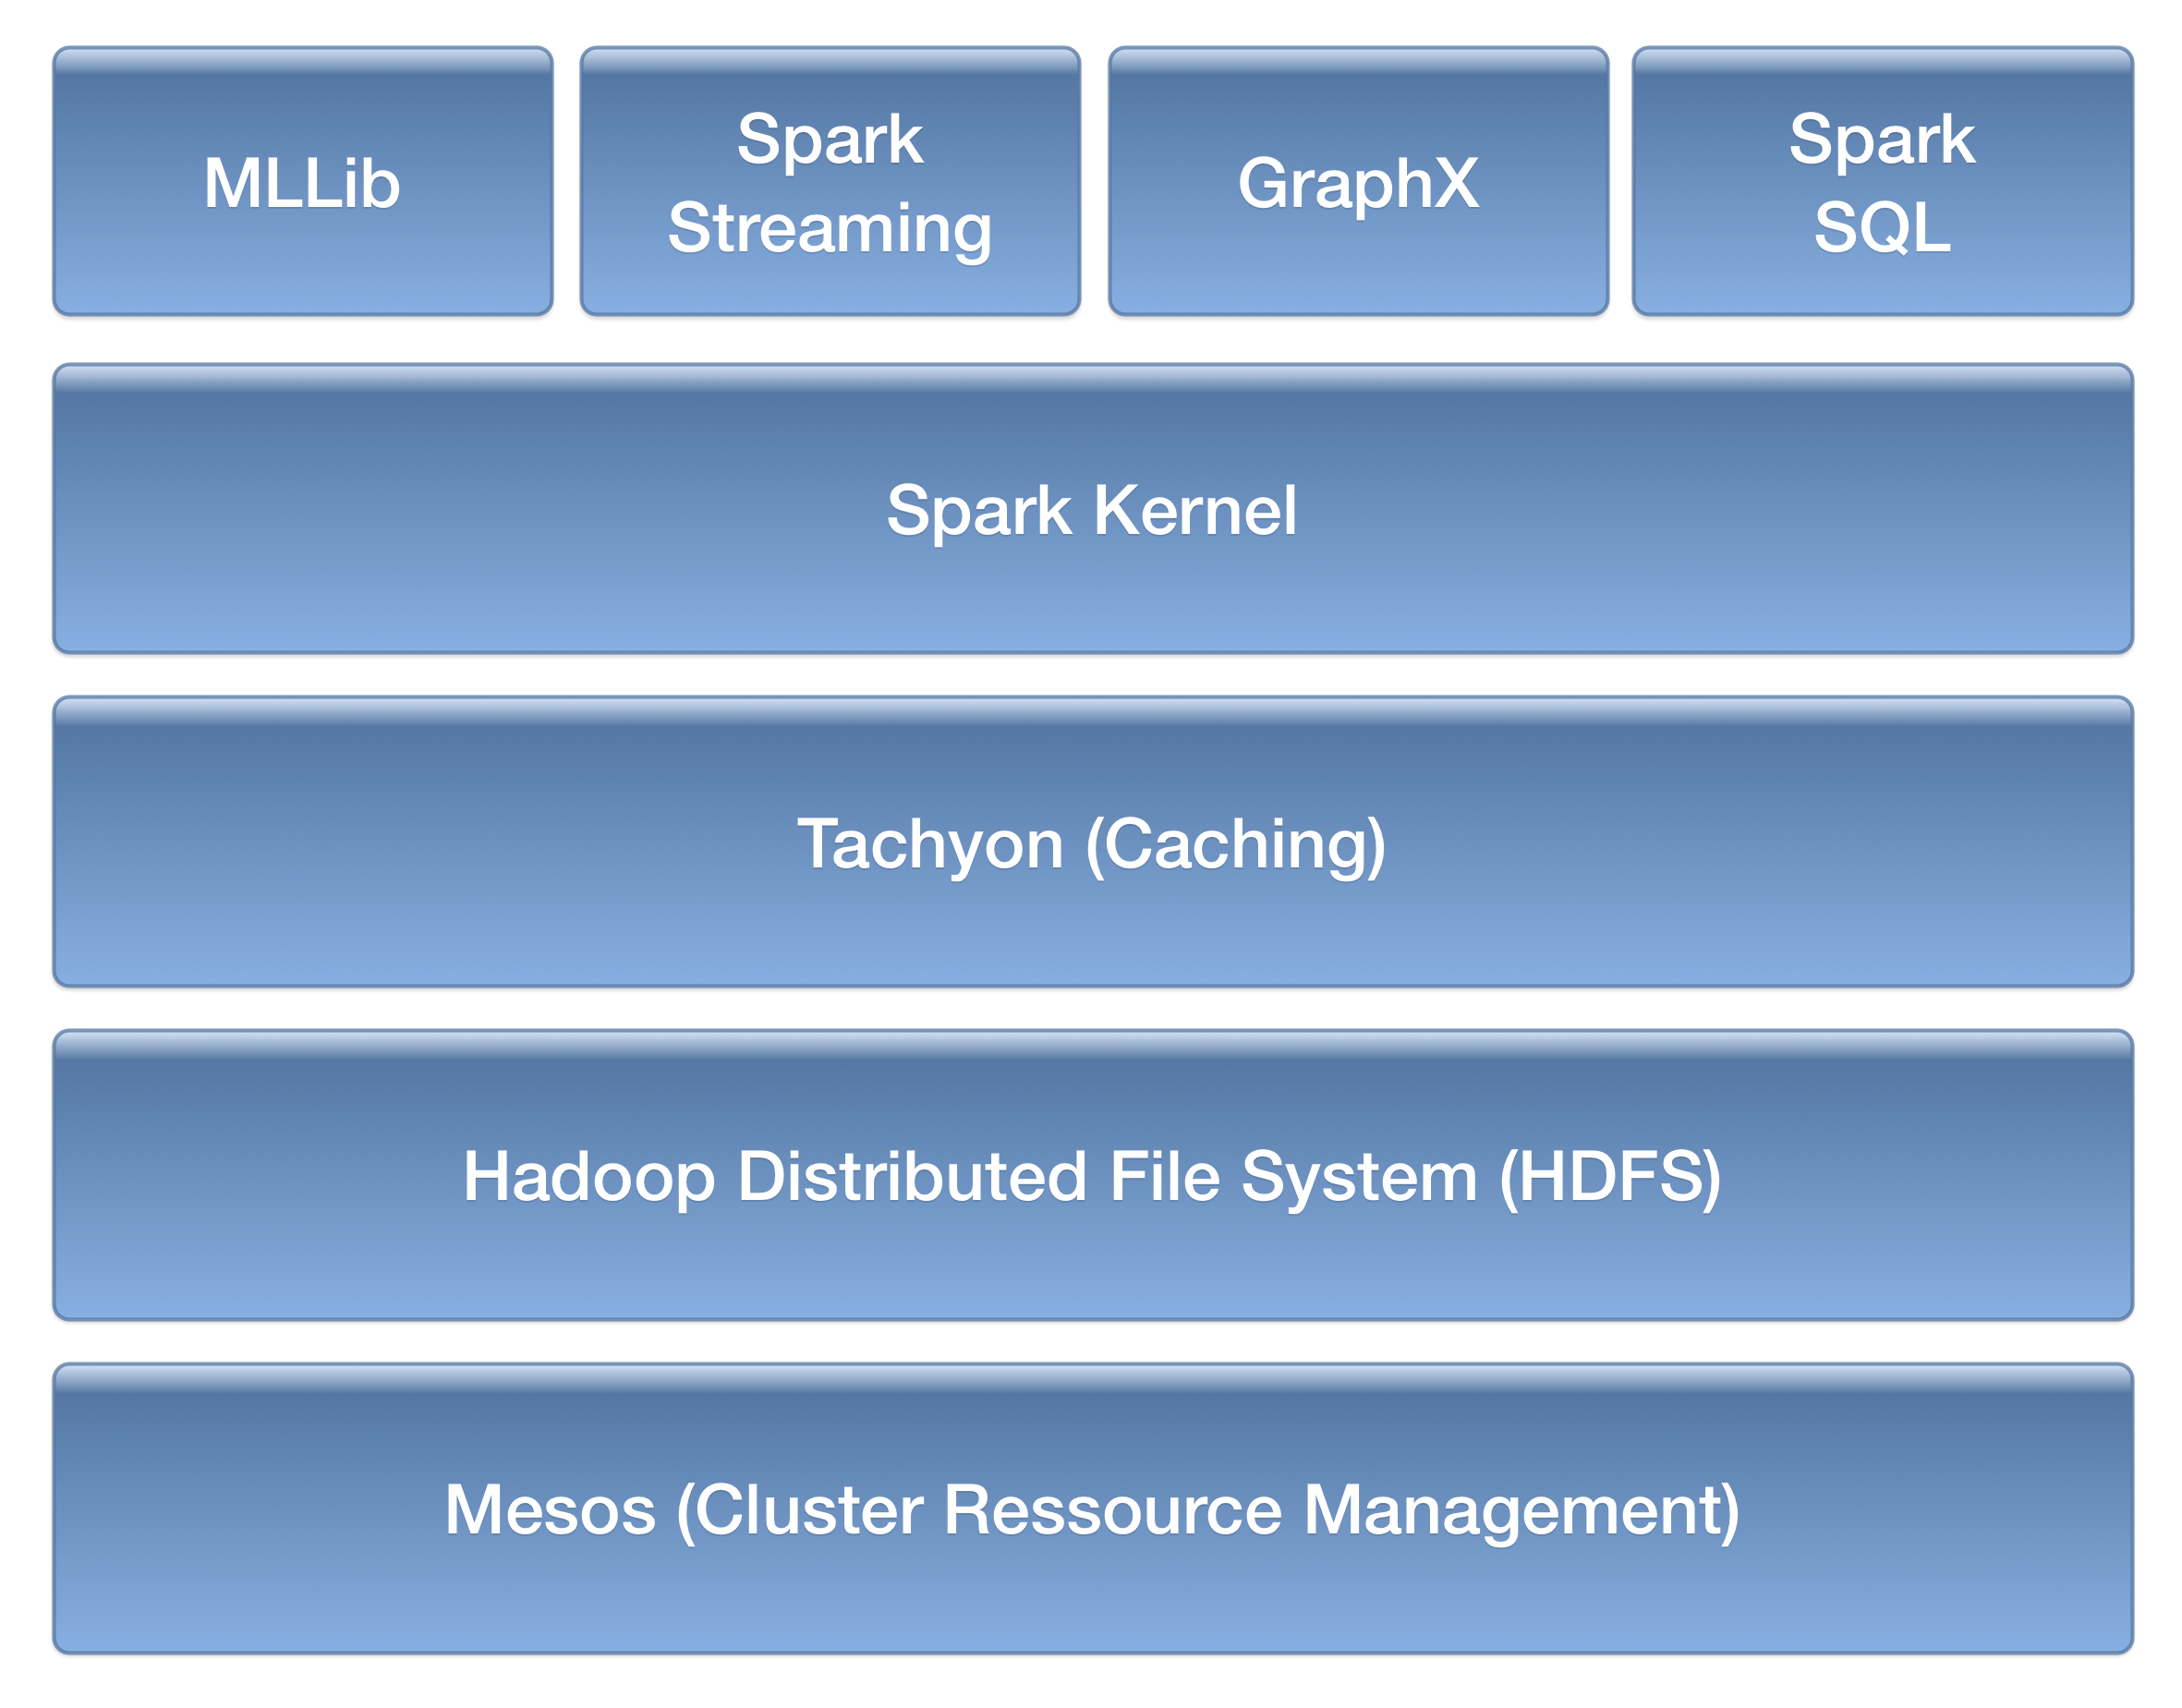
\includegraphics[width=1.0\textwidth]{bilder/BDAS.png}
\caption{Übersicht des BDAS mit den vom AMPLab empfohlenen Bibliotheken.}
\label{fig:BDAS1}
\end{figure}
 


In Abbildung \ref{fig:bdas]} ist der Aufbau des BDAS nochmals schematisch dargestellt. Die grün hinterlegten Elemente markieren die Bestandteile des aktuellen BDAS, die violett hinterlegten zeigen alternative Implementierungen auf der jeweiligen Schicht. Grün schraffiert ist die Applikationsschicht, wo Applikationen oberhalb von Spark und den direkten Anwendungen angesiedelt sind. 

\begin{figure}[htb!]
\centering
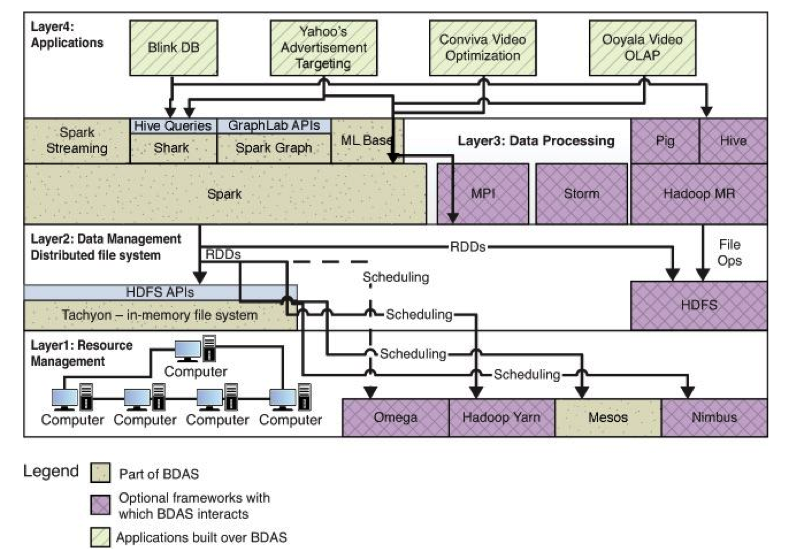
\includegraphics[width=1.0\textwidth]{bilder/2_2_stack.png}
\caption{Der BDAS. Abbildung aus „Big Data Analytics Beyond Hadoop“, S 15 \protect\citelit{va14}}
\label{fig:bdas]}
\end{figure} 


\section{Apache Mesos}
\label{section:apache Mesos}


Bei \textit{Apache Mesos} handelt es sich um ein \textit{Cluster-Management-Framework} für Anwendungen, die in verteilten Serverpools laufen sollen. Bestandteil von Mesos ist wiederum \textit{Apache ZooKeeper}, das für Konfigurationsinformationen, Naming-Services und die Synchronisation von verteilten Anwendungen zuständig ist.  

Mesos wird im BDAS eingesetzt, um die Prozesse von Hadoop/Spark effizient auf die einzelnen Knoten im Cluster zu verteilen. Besonders das Ressourcen-Management und –Monitoring innerhalb des Clusters ist ein wichtiger Faktor, um Jobs performant auf verteilten Systemen ausführen zu können. Auch das Fehlerhandling für Knoten, Prozesse und im Netzwerk wird im Berkeley-Stack von Mesos übernommen. 

Ein besonderer Vorteil von Mesos gegenüber Yarn oder anderen Alternativen, wie dem Cloudera Cluster Manager oder Ambari von Hortonworks ist die Möglichkeit, verschiedene Frameworks gleichzeitig und isoliert in einem Cluster betreiben zu können. So kann beispielsweise Hadoop mit Spark in einer gemeinsamen Infrastruktur koexistieren.   
	
\section{Hadoop Distributed File System (HDFS) und Tachyon}
\label{section:hadoop Distributed File System (HDFS) und Tachyon}


Das Hadoop Distributed File System basiert ideologisch auf dem GoogleFileSystem (GFS) und hat zum Zweck, zuverlässig und fehlertolerant sehr große Dateien über verschiedene Maschinen hinweg in verteilten Umgebungen zu speichern. In entsprechenden Veröffentlichungen von Hortonworks \citeint{ho14} wird von Produktivsystemen berichtet, die bis zu 200 PetaByte an Datenvolumen in einem Cluster von 4500 Servern basierend auf HDFS verwalten.

HDFS wurde speziell für den Einsatz mit MapReduce entwickelt, ist also auf geringe Datenbewegungen ausgelegt, da MR die Berechnungsprozesse jeweils zu den physischen Datensätzen selbst bringt und nicht, wie herkömmlich, die Daten zu den Prozessen geliefert werden müssen. So wird massiv Netzwerkverkehr innerhalb des Clusters eingespart und letztlich werden nur Prozesse und Prozessergebnisse verschickt.  

Die Hauptbestandteile von HDFS sind der sogenannte NameNode, der die Metadaten des Clusters verwaltet und die DataNodes, die die eigentlichen Daten halten. Dateien und Verzeichnisse werden vom NameNode durch inodes repräsentiert. Diese wiederum enthalten Informationen über Zugriffsrechte, Zugriffszeiten oder Größenangaben der Dateien.



\begin{figure}[htb!] 
\centering
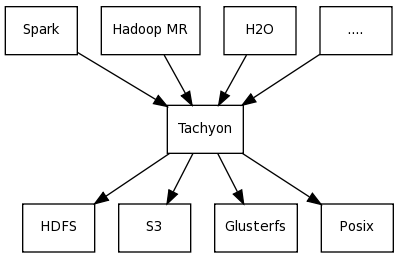
\includegraphics[width=1.0\textwidth]{bilder/2_3_stack.png}
\caption{Der Datamanagement-Layer im BDAS mit HDFS und Tachyon}
\label{fig:datamgmtlayer}
\end{figure} 

 

In Abbildung \ref{fig:datamgmtlayer} wird die Datenmanagementschicht des BDAS nochmals detaillierter dargestellt. Hier ist erkennbar, dass reine Hadoop-Implementierungen direkt auf dem HDFS aufsetzen, da das HDFS für \textit{MapReduce} optimiert ist. 

Kommt hingegen Spark zum Einsatz, lässt sich wahlweise direkt das \textit{HDFS} ansprechen oder alternativ eine Zwischenschicht nutzen, die auf das In-Memory-Modell von Spark zugeschnitten ist. Dies ist innerhalb des BDAS das verteilte Dateisystem Tachyon. Hier werden die zu verarbeitenden oder zu analysierenden Datensätze direkt in den Hauptspeicher des jeweiligen Knoten in Form eines Cache gehalten. Somit werden Lade- und Speicheroperationen auf Massenspeicher minimiert und eine massiv höhere Ausführungsgeschwindigkeit erreicht. Unterhalb von Tachyon ist nach wie vor ein HDFS für die persistente Datenhaltung notwendig. Alternativ kann auch das Amazon S3-File-System eingesetzt werden. Tachyon wurde direkt innerhalb der AMPLabs entwickelt und ist mittlerweile fester Bestandteil des BDAS.  


\section{Apache Spark}
\label{section:apache Spark}

Spark ist das Herzstück des BDAS. Bei Spark handelt es sich um ein open-source Data-Analytics-Framework, das, wie Hadoop, speziell für die Bedürfnisse im Rechner-Cluster konzipiert ist. Auch Spark nutzt das HDFS entweder direkt, oder indirekt über Tachyon. Im Gegensatz zu Hadoop bietet Spark jedoch Funktionen für In-Memory-Cluster-Berechnungen und ist nicht zwingend an MapReduce gebunden. Besonders interaktive Analyse oder Verarbeitung der Daten, Abfragen über verteilte Dateien und iterative 

Lernalgorithmen erfahren so laut AMPLab eine bis zu hundertfache Ausführungs-geschwindigkeit im Gegensatz zu Hadoop. Auch die im ersten Kapitel angesprochenen Schwächen von Hadoop bei Berechnungen von komplexen linear-algebraischen Problemen, generalisierten n-Körper-Problemen, diversen Optimierungsproblemen und diversen anderen Aufgaben, treten bei Spark auf Grund der offenen Architektur und der Zerlegung von Datensätzen in die sogenannten Resilient Distributed Datasets (RDD) nicht mehr auf.

Spark wurde komplett in Scala entwickelt und bietet APIs für Scala, Java (inklusive Lambda-Expressions von Java 8) und Python. Im Labor existieren bereits Spark-Installationen mit bis zu 2000 Knoten, in Produktivsystemen sind bisher Systeme mit bis zu 1000 Knoten im Einsatz \citeint{cm13}. Durch die Möglichkeit, die Datensätze im Speicher für interaktive Analyseaufgaben zu cachen und iterativ abzufragen, ist eine direkte Kommandozeileninteraktion über das integrierte Scala REPL (alternativ auch in Python) möglich. 

Für Spark existieren dedizierte Bibliotheken für Verarbeitung von Datenströmen, Machine-Learning und Graphenverarbeitung. Ähnliche Artefakte existieren auch für Hadoop (Mahout, Vowpal Wabbit, etc.), jedoch ist die Architektur von Spark wesentlich besser für derartige Anwendungsbereiche zugeschnitten. 
   
\section{Spark Streaming}
\label{section:spark Streaming}


Spark Streaming ist eine der oben genannten Bibliotheken, die Spark um dedizierte Anwendungsbereich erweitert. Hierbei handelt es sich um eine Erweiterung, um die integrierte API von Spark für Anwendungen auf Datenströmen nutzen zu können. Das Programmiermodell unterscheidet nicht zwischen Batch- und Streaming-Anwendungen. So lassen sich beispielsweise Datenströme zur Laufzeit mit Archivdaten vergleichen und direkt Ad-hoc-Abfragen auf die Ströme formulieren. Im Fehlerfall ermöglicht Streaming zahlreiche Wiederherstellungsoptionen, sowohl von verlorenen Datenströmen, als auch von Einstellungen. Ein Anwendungsbeispiel ist die Echtzeitanalyse von Twitter-Meldungen. 

\section{GraphX}
\label{section:graphX}


GraphX ist eine Erweiterung für Spark, die verteilte, flexible Graphen-Anwendungen in einem Spark-Cluster ermöglicht \citeint{xg13}. Besonders in den Disziplinen „Machine Learning“ und „Data Mining“ ist die Anwendung komplexer Graphen unerlässlich. Graph-datenbanken kommen immer dann zum Einsatz, wenn stark vernetzte Informationen und ihre Beziehungen zueinander interessant sind. Hier werden die Entitäten als Knoten behandelt, die Beziehungsart definiert die Kanten. Die Kanten können auch gewichtet 

sein. Ein konkretes Beispiel sind die Mitglieder eines sozialen Netzwerks mit ihrem jeweiligen Beziehungsgeflecht. Je nach Kontaktintensität können diese Beziehungen auch priorisiert werden, was hier dem Kantengewicht entspricht.

GraphX nutzt hier die Vorteile der darunterliegenden Spark-Infrastruktur, in dem durch eine tabellarische Anordnung der Datenstrukturen eine massive Parallelisierung möglich ist und auch der Verarbeitung in RDDs voll unterstützt wird. So sind auch interaktive Operationen auf den Graphen jederzeit über REPL möglich. 

\section{MLbase/MLLib}
\label{section:mLbase/MLLib}


MLbase ist eine Sammlung von Bibliotheken und Werkzeugen für Machine-Learning-Anwendungen mit Spark. Sie besteht grundsätzlich aus den drei Teilen MLlib, MLI und ML-Optimizer und ist oberhalb der Spark-Installation angesiedelt, wie auf Abbildung \ref{fig:mlbase} zu erkennen ist. 

\begin{figure}[htb!]
\centering
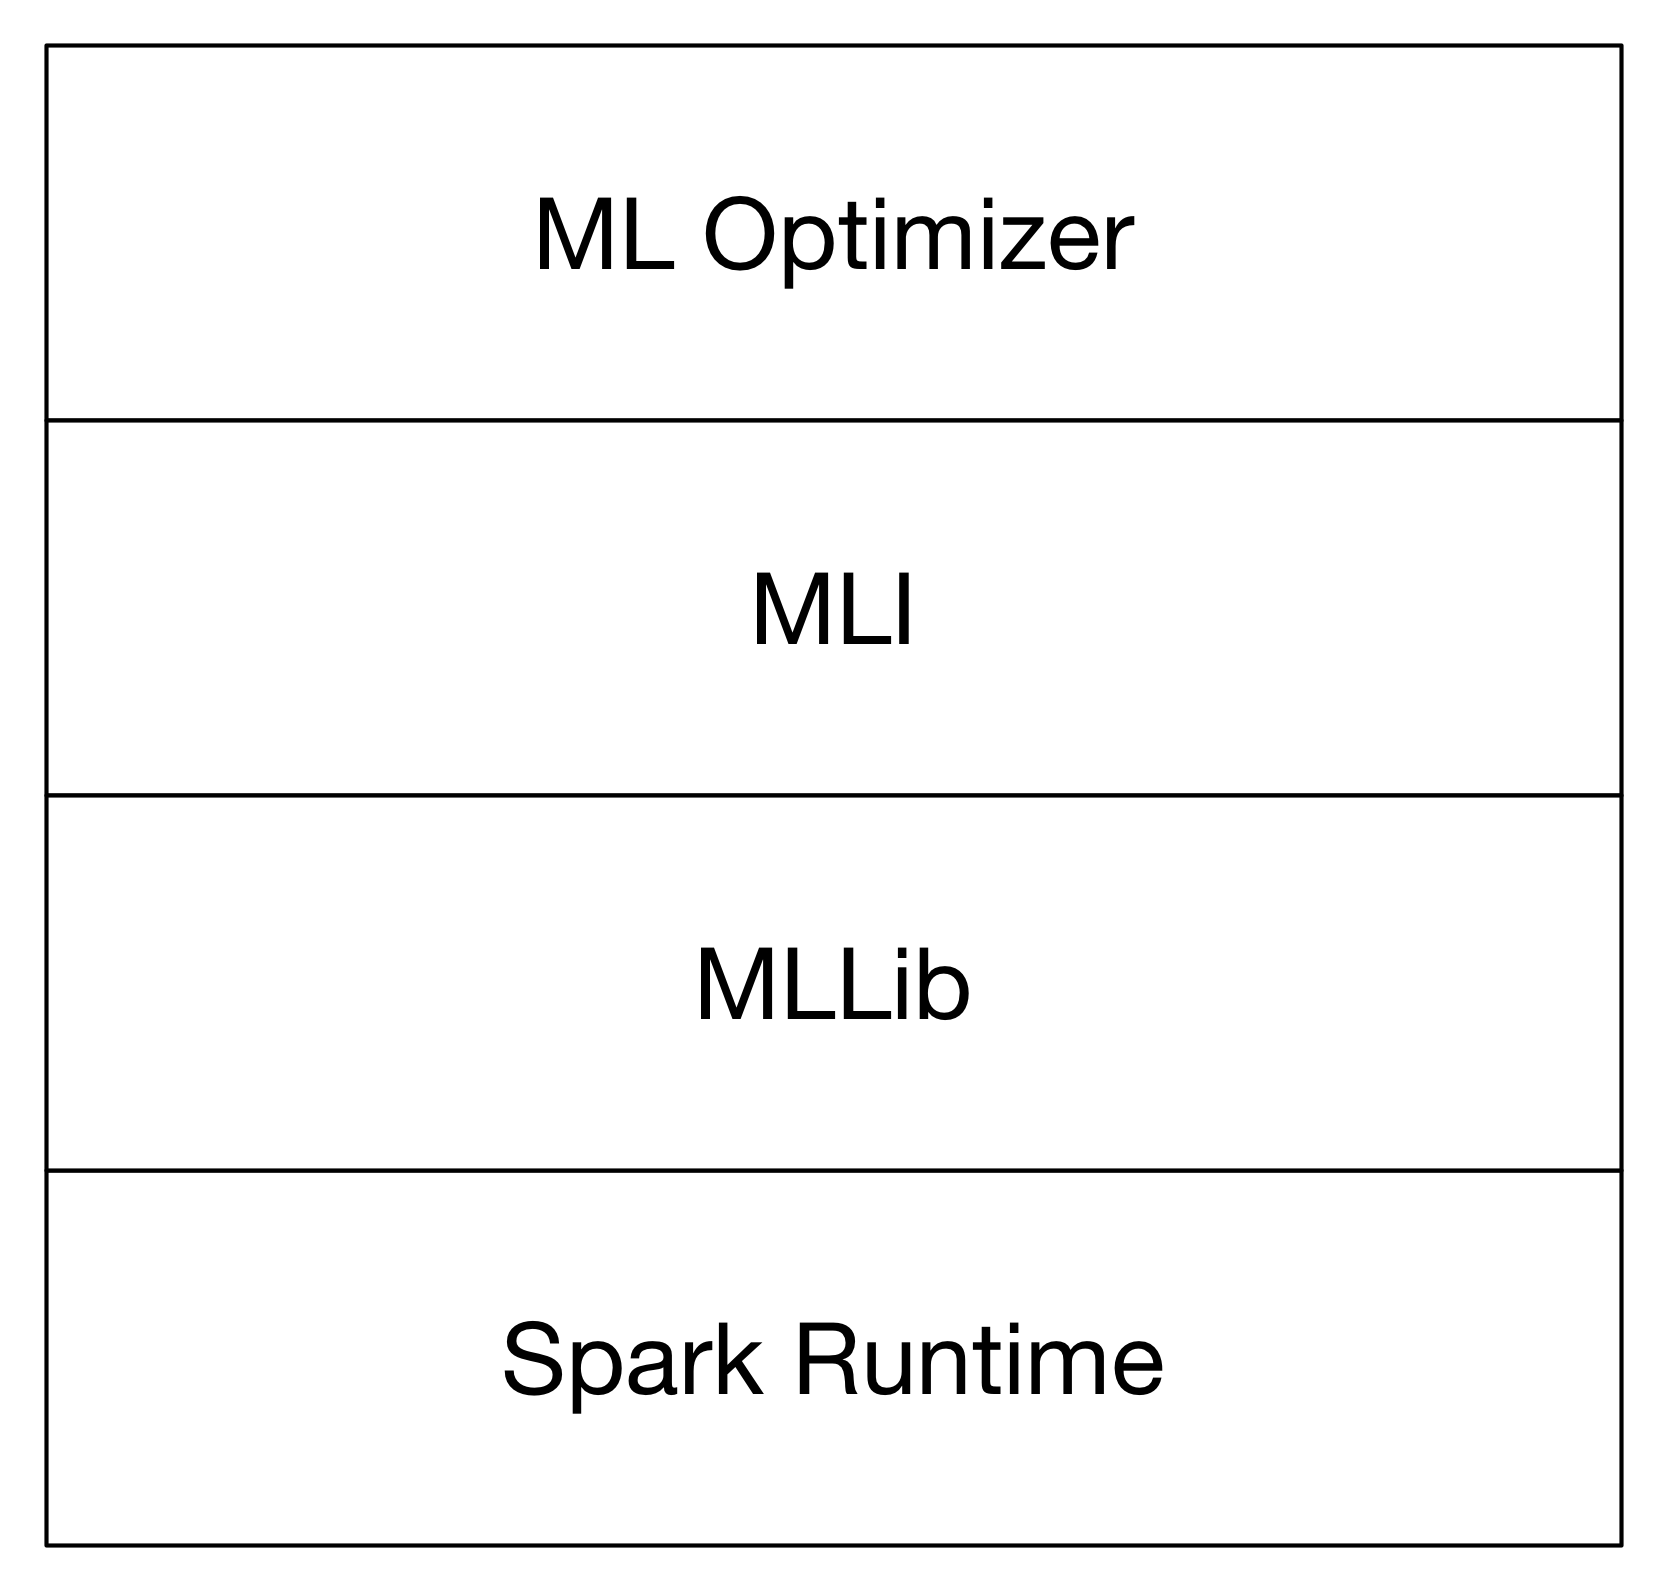
\includegraphics[width=1.0\textwidth]{bilder/2_4_3_mlbase.png}
\caption{Die Bestandteile der MLbase \protect\citeint{ml10}}
\label{fig:mlbase}
\end{figure} 
 


Die MLlib ist eine verteilte Machine-Learning-Bibliothek die für die Spark-Laufzeitumgebung entwickelt wurde und die bekannten Algorithmen für Probleme wie Klassifikation, Regression, Clustering und kollaboratives Filtern enthält.

Bei MLI handelt es sich um eine API, die es ermöglicht, selbst ML-Features zu entwickeln und in erster Linie für komplexere Problemstellungen geeignet ist. Mit MLI lassen sich die Funktionen direkt gegen Spark entwickeln, gegebenenfalls unter Zuhilfenahme der Bibliotheken der MLlib.

Der ML-Optimizer soll ML-Probleme für Endnutzer vereinfachen, in dem Modellauswahlen automatisiert werden. Hierzu werden Features aus der MLlib und der MLI extrahiert und zur Hilfe genommen.



\section{Spark SQL}
\label{section:spark SQL}


\textit{Hive} ist eine \textit{SQL-Query-Engine} für Hadoop, die sich großer Beliebtheit in der Hadoop-Community erfreut. Spark SQL\footnote{Ursprünglich war die für den BDAS-Stack empfohlene Implementierung einer SQL-Query-Engine unter dem Namen \textit{Shark} bekannt. Im Juli 2014 wurde jedoch bekanntgegeben, dass die Entwicklung von Shark zugunsten von Spark SQL eingestellt wurde und die vorhandenen Shark-Implementierungen voll in Spark SQL integriert werden. Deshalb zeigen Schaubilder des BDAS von vor Juli 2014 Shark als Query-Engine.} ist eine Portierung dieser Engine für Spark, um alle Vorteile der BDAS-Architektur nutzen zu können und ist kompatibel mit sämtlichen Hive-Daten, -Metastores und –Queries. Im Gegensatz zu Hive, das aus Datensätzen zur Laufzeit Java-Objekte generiert, nutzt Spark SQL eine zeilenorientierte Speicherung mittels Arrays primitiver Datentypen und ist somit selbst in einer Hadoop-Infrastruktur im Mittel bis zu fünfmal schneller als Hive. 

Eine Besonderheit von Spark SQL ist neben seinem SQL-Interface die Möglichkeit, auch Machine-Learning-Funktionen als Abfragen formulieren zu können. 

Für die Anwendung von Spark SQL hat sich die Architektur von Spark mit seinen RDDs als sehr vorteilhaft erwiesen, da Abfragen auf Fehlerhaften RDDs nach dem Neuaufbau des entsprechenden Datasets direkt erneut ausgeführt werden können. 

Ein weiterer Unterschied zu Hive ist die sogenannte Partial-DAG-Execution (PDE). Dies bedeutet, dass logische Abfragepläne in Spark SQL aufgrund gesammelter Statistiken zur Laufzeit flexibel erstellt werden im Gegensatz zu Hive oder herkömmlichen relationalen Datenbanksystemen, wo bereits zur Kompilierungszeit starre physische Abfragepläne generiert werden. Besonders die Machine-Learning- und Failover-Funktionen wären mit einer Planerstellung zu Kompilierzeit nicht umsetzbar. 






\subsection{Zusammenfassung}
\label{section:storm}





\chapter{Funktionsweise von Spark}
\label{chapter:funktionsweise von Spark}


Im vohergehenden Kapitel wurde der Berkeley Data Analytics Stack vorgestellt. Es wurde gezeigt, dass dieser aus einer Reihe von Bibliotheken, Infrastrukturkomponenten und dem eigentlich Kern, Apache Spark, besteht.

In diesem Kapitel werden die grundlegenden Konzepte von Spark vorgestellt und dessen Funktionsweise betrachtet. Einleitend wird gezeigt, wie eine Spark-Infrastruktur aufgebaut sein kann, wie diese intern Abfragen und eigene Spark-Programme verarbeitet und wie der \textit{Spark-Context} sich als Cluster-Repräsentant gegenüber dem Anwender und der API exponiert. Im nächsten Unterkapitel wird die eigentliche Basis von Apache Spark vorgestellt. Spark basiert im Wesentlichen auf einer verteilten Datenstruktur, den \textit{Resilient Distributed Datasets}. Deren Konzept wird sowohl theoretisch, als auch im Anwendungskontext dargestellt. 

Ein weiteres Kernelement der Spark-Implementierung bildet das \textit{In-Memory-Processing} der Daten. Spark ist in der Lage, je nach Konfiguration des Host-Systems, große Teile der Analysen und Verarbeitungen äußerst flexibel im Hauptspeicher durchzuführen und so massive Performanceverbesserungen gegenüber festspeicherbasierter Verarbeitung zu generieren. Hierzu bietet Spark spezielle \textit{In-Memory-Primitives} an. In einem weiteren Unterkapitel werden dieses detailliert vorgestellt. 



\section{Spark im Cluster}
\label{section:spark im cluster}

%Diesen Abschnitt noch mit Referenzen untermauern
Eine große Herausforderung im Umfeld verteilter und nebenläufiger Analyse und Verarbeitung großer Datenmengen stellt der Netzwerkverkehr da. Der klassische Aufbau einer verteilten Anwendung hält die Daten auf einer dafür vorgesehen Plattform im Netzwerk. Häufig ist dies ein dedizierter File- oder Datenbankserver, der mit möglichst großer Bandbreite mit dem Applikationsserver verbunden ist (Vergleich Oracle InfinyBand). 

%Hier muss noch eine Grafik eines herkömmlichen Netzwerks rein
\begin{figure}[htb!]
\centering
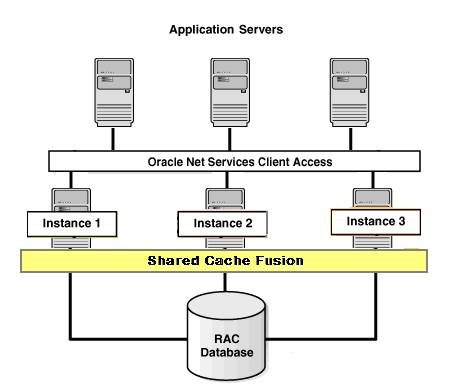
\includegraphics[width=1.0\textwidth]{bilder/oracle_cluster.jpg}
\caption{Aufbau eines Standardcluster im Rechenzentrumsbetrieb mit Application-Server und Oracle Datenbanken \protect\citeint{or14}. }
\label{fig:sparkclustermastermitworker}
\end{figure} 

In diesem Aufbau entsteht in der Regel eine sehr hohe Netzwerklast, da die für die Applikation benötigten Daten dieser zunächst zur Verfügung gestellt werden müssen. 

Spark geht hier einen anderen Weg. Ein Spark-Cluster besteht typischerweise aus einem zentralen \textit{Master} und n \textit{Worker-Nodes}. Diese können aus einfachen Servern bestehen, aber auch aus Clustern von Großrechnern (beispielsweise IBM Z, Oracle Exa). Das Hadoop Distributed File System und Spark skalieren über Cluster beliebiger Größenordnung. Über ein verteiltes Dateisystem werden die Daten auf dem Cluster gehalten und sowohl dem \textit{Master}, als auch den \textit{Worker-Nodes} so zur Verfügung gestellt. 

%Hier Grafik zum Aufbau eines Spark Clusters. 
\begin{figure}[htb!]
\centering
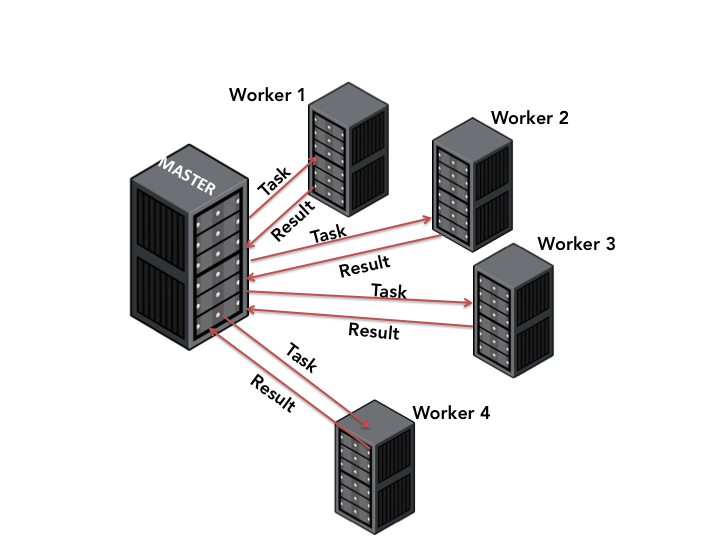
\includegraphics[width=1.0\textwidth]{bilder/spark1.png}
\caption{Clusteraufbau mit Spark mit einem Master und vier Worker-Nodes. }
\label{fig:sparkclustermastermitworker}
\end{figure} 



Spark-Anwendungen laufen als unabhängiges Set von Prozessen auf Cluster-Infrastrukturen. Das Hauptprogramm, der sogenannte \textit{Spark Driver}, instanziert das\textit{ SparkContext-Objekt}, das die einzelnen Prozesse koordiniert. Auf Clustersystemen hält der \textit{SparkContext} die Verbindung zum jeweiligen \textit{Cluster-Ressource-Manager} (Mesos, Yarn), im Standalone-Betrieb instanziert der Context selbst einen Dummy-Manager und allokiert in beiden Fällen die für die Anwendung nötigen Hardware-Ressourcen. Die Cluster-Manager liefern ihren aktuellen Status an Spark zurück und melden Auslastung und Gesundheitszustand der einzelnen Knoten. Über interne \textit{Load-Balancing-Systeme}\footnote{Load-Balancing-Systeme sind Überwachungsmechanismen in verteilten Systemen. Jedes Teilsystem meldet seine eigene Auslastung und seine Verfügbarkeit an den Load-Balancer. Dieser verteilt anstehenden Aufgaben so auf die Ressourcen, dass eine möglichst gleichmäßige Verteilung über die gesamte Infrastruktur möglich ist.} wird ermittelt, welche Worker-Nodes die jeweiligen Tasks aus dem Spark-Kontext zugewiesen bekommen. Der SparkContext repräsentiert sowohl für die Spark-Konsole REPL, als auch in eigenen Spark-Programmen innerhalb der APIs das gesamte Cluster. Dem SparkContext wird bei der Initialisierung über ein Konfigurationsobjekt mitgeteilt, welche Ressourcen ihm für das aktuelle Programm zur Verfügung stehen. Die Entscheidung, welche, der initial zur Verfügung gestellten Nodes oder Ressourcen des Clusters von Spark wann in Anspruch genommen werden, obliegt der Kombination aus Spark und \textit{Cluster-Ressource-Manager}. 

%gesamten Abschnitt mit Referenzen belegen!    

%fußnote nochmal überdenken

\begin{figure}[htb!]
\centering
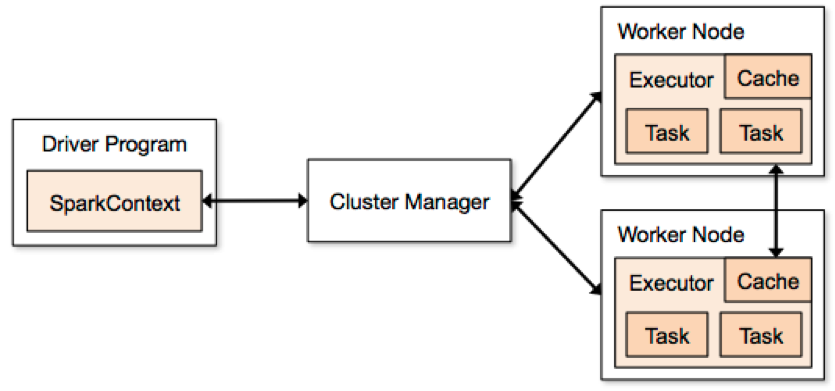
\includegraphics[width=1.0\textwidth]{bilder/3_2_cluster.png}
\caption{Clusteraufbau mit Spark \protect\citeint{sp14}}
\label{fig:sparkcluster}
\end{figure} 





Wenn ein SparkContext initialisiert wurde, installiert der Spark sogenannte \textit{Executors} auf sämtlichen Worker-Nodes des Clusters. Der Applikationscode wird nun als JAR\footnote{Ein JAR (Java ARchive) ist ein gepacktes und auf einer Java Virtual Machine ausführbares (Java, Scala, Clojure) Programmpaket, häufig inklusive der benötigten Bibliotheken.} direkt an die Executors verteilt und dieser anschließend durch entsprechende Tasks ausgeführt. 



  
\section{Das Konzept der Resilient Distributed Datasets}
\label{section:rdd}

Die Resiliient Distributed Datasets (RDD) sind das eigentliche Kernelement von Apache Spark. Hierbei handelt es sich um fehlertolerante, parallele Datenstrukturen, die dem Anwender erlauben, Zwischenergebnisse explizit im Hauptspeicher zu halten, ihre Partitionierung zu steuern, um Daten bewußt an bestimmten Stellen halten zu können und diese mittels umfangreichen Operatoren zu manipulieren  \citelit{rdd12}. Das Konzept der RDDs entspricht prinzipiell den Views\footnote{Eine View ist in einem relationalen Datenbanksystem die Ergebnismenge einer persistierten Datenbankabfrage auf bestimmte Daten. Diese lässt Abfragen analog zu einer gewöhnlichen Tabelle zu.} in relationalen Datenbanksystemen. Werden die RDDs für weitere Zugriffe persistiert, enspricht dies dem Prinzip der Materialized Views\footnote{Materialized Views entsprechen bei Abfragen den regulären Views. Allerdings wird hier im Gegensatz zu den Views bei Zugriff keine Abfrage auf die zugrundeliegenden Tabellen durchgeführt. Stattdessen sind die Daten als Kopie in eigenen Datenbankobjekten persistent vorhanden.}.  

RDDs werden mittels deterministischer, paralleler Operationen erstellt, den sogenannten \textit{Transformationen}. Im Fehlerfall, also wenn beispielsweise ein \textit{Node} im Cluster ausfällt, können die RDDs automatisch an Hand der durchgeführten Regeln neu aufgebaut werden. Deshalb merken sich die RDDs die Transformationen, die zu ihrem Aufbau geführt haben und können so verlorene Datenstrukturen schnell rekonstruieren. Die \textit{Resilient Distributed Datasets} können ausschließlich durch Transformationen, wie beispielsweise \textit{map, filter, join}, etc., aus Daten aus dem Dateisystem oder aus anderen, bereits vorhandenen RDDs erzeugt werden, oder durch Verteilen einer Object-Collection in der Driver-Applikation. Diese Datenstrukturen müssen nicht persistiert werden, da sie für einen Partitionierung ausreichende Informationen über ihre Erstellungsregeln und die entsprechenden Datensätze enthalten, das sogenannte \textit{Lineage} \citelit{rdd12}.   

Da es sich bei RDDs prinzipiell um Scala-Collections handelt, können diese auch direkt in Scala-Code eingebunden und verarbeitet werden, oder interaktiv über die Scala-Konsole REPL genutzt werden. Aber auch für Java und Python bietet Spark APIs an. Für weitere Sprachen wie R oder Clojure existieren Wrapper-Frameworks, welche die RDDs und ihre Operationen verfügbar machen.  RDDs können nur durch grobgranulare, deterministische Transformationen, erstellt werden.

WIe eingangs beschrieben, verfügen die Anwender von Spark über die Kontrolle der Aspekte \textit{Persistence} und \textit{Partitioning} \citelit{rdd12}. Mit der Persistence lässt sich festlegen, welche RDDs wiederverwendet werden sollen, also welche RDDs nach welcher Strategie persistiert werden sollen. Das Partitioning legt fest, nach welchen Kriterien die RDDs geteilt und über das Cluster verteilt werden sollen, also beispielsweise sortiert nach bestimmten Keys. Die Optimierung der Partitionierung ist unter Anderem wichtig für Join-Operationen. Je nach Partitionierungsstrategie kann dies erhebliche Unterschiede in Laufzeit und Ressourcennutzung bedeuten.  

RDDs können prinzipiell auf drei Arten gespeichert werden \citeint{sp14}:
\begin{itemize}
		\item Als deserialisiertes Java-Objekt im Speicher der JVM – dieses Variante bietet die beste Performance, da die Objekte sich direkt im JVM-Heap befinden
		\item Als serialisiertes Java-Objekt direkt im Speicher – dieses Verfahren ist speicher-effizienter, aber schlechter in der Zugriffsgeschwindigkeit
		\item Im Dateisystem – diese Variante ist erwartungsgemäß die langsamste, jedoch nötig, wenn die RDDs zu groß für die Haltung im RAM sind. 		
\end{itemize}	


\begin{tabular}{ l l c | r |}
\hline
test1 test2 test3
\end{tabular}


Wie in Abbildung \ref{section:rdd} dargestellt, werden die Daten bei einer Verarbeitung durch Spark zunächst aus dem HDFS geladen, in Resilient Distributed Datasets (RDD) verpackt, und dann im Hauptspeicher für Verarbeitung- oder Analysefunktionen zur Verfügung gestellt. Abfragen werden direkt entweder via Scala REPL oder SQL-artige Abfragen zur Laufzeit, über Batch-Jobs oder via Spark Streaming/Storm an die im RAM befindlichen RDDs geleitet.

\begin{figure}[htb!]
\centering
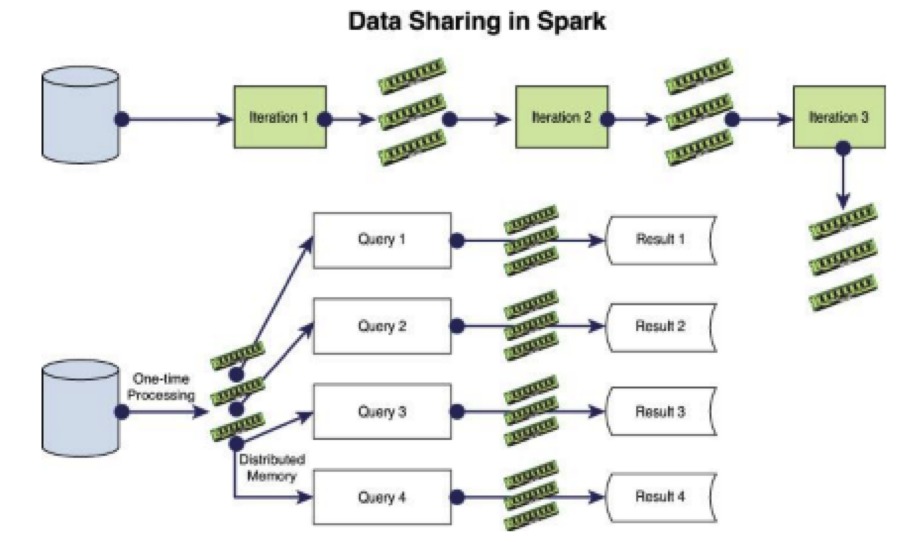
\includegraphics[width=1.0\textwidth]{bilder/3_spark.png}
\caption{Schematische Darstellung der Funktionsweise von Spark \protect\citeint{va14}}
\label{fig:sparkfunkt}
\end{figure}



\section{Die In-Memory-Primitives von Spark}
\label{section:rdd}


\section{Die Spark-Console REPL}
\label{section:rdd}


\section{Die Spark APIs}
\label{section:rdd}



























\chapter{Exemplarischer Architekturaufbau und Inbetriebhnahme einer Apache Spark Infrastruktur }
\label{chapter:architektur}



Im folgenden Kapitel wird ein exemplarischer Architekturaufbau eines lokalen Entwicklungs- und Testsystems für Apache Spark vorgestellt. Wie in den vorangegangen Kapiteln gezeigt wurde, handelt es sich bei Spark in erster Linie um ein Framework für leistungsstarke Clustersysteme. Dennoch muss Spark auch auf entsprechend kleiner dimensionierten System betrieben werden können. Häufig ist in einem professionellen Umfeld beispielsweise nur ein Cluster für Produktionsaufgaben vorhanden, die Test- und vor allem auch die Entwicklersysteme stellen sich häufig in Form sogenannter \textit{SIngle-Node-Cluster} dar. 

Besonders der Aspekt der Entwicklungsarbeitsplätze rückt hier in den Vordergrund. Da Spark lediglich über den Master-Node und hier über den Spark-Context innerhalb des Driver-Program für die Entwickler zugreifbar ist und die interne Verteilung der Tasks auf die jeweiligen Nodes von Spark und den Clustermanagement-Systemen übernommen und maskiert wird, stellt sich die Fehleranalyse mittels klassischem \textit{Debugging}\footnote{Unter klassischem Debugging wird hier das Setzen von Breakpoints und das explizite Überwachen von Variablenwerten zur Laufzeit durch Entwickler verstanden.} als sehr große Herausforderung dar. 

\section{Ausführungscontainer: Docker}
\label{section:docker}

\section{Cluster Management: Mesos und Yarn }
\label{section:mesos}

Blablba

\section{Caching-Framework: Tachyon}
\label{section:tachyon}

Blablba

\section{Der eigentliche Kern: Apache Spark}
\label{section:kern}

Blablba

\section{Streaming-Framework: Spark Streaming}
\label{section:streaming}

Blablba

\section{Abfrageschicht: Spark SQL}
\label{section:spark sql}

Blablba

\section{Machine Learning Algorithmen: MLLib}
\label{section:mllib arch}

Blablba



\section{Graphenanwendungen: GraphX}
\label{section:graphx}

Blablba


\chapter{Implementierung der Prototypen }
\label{chapter:implementierung}



Im vorherigen Kapitel wurde gezeigt, wie verschiedene Entwicklungs- und Testinfrastrukturen mit Apache Spark aufgesetzt werden können. Im Rahmen dieser Thesis wurden für die Frameworks Spark und Flink, sowie für MLLib und H2O jeweils ein Prototyp für Vergleichsmessungen erstellt. Darüber hinaus wurden kleinere Testprototypen für die Bibliotheken Spark Streaming, sowie für GraphX erstellt. Diese werden im folgenden Kapitel vorgestellt.  

\section{Prototyp: Spark}
\label{section:prototyp spark}

Das Framework Apache Spark bietet durch seine APIs umfangreiche Möglichkeiten der applikatorischen Datenanalyse und Manipulation. Besonders Anwendungen auf große, persistierte Datenmengen lassen sich so komfortabel mittels Batch-Processing analysieren und verarbeiten. 

Deshalb wurde zum Test der Frameworks Apache Spark und Flink auf eine möglichst große Datenbasis zurückgegriffen, auf der einige durch die APIs angebotene elementare Funktionen angewendet werden.  

Zunächst wurde eine unstrukturierte Textdatei mit einer Größe von ca. 5 GB erstellt. Aus diesen Daten erstellt Spark ein RDD, verteilt es innerhalb der vorhandenen Infrastruktur und zählt alle vorkommenden Buchstaben "e" und "s". 
Das folgende Listing zeigt diese Testanwendung in Scala.

\newpage

\begin{lstlisting}[label=vwikilogs,caption=SimpleTestApp.scala - zählt Buchstabenvorkommen in Textdateien.]
 /* SimpleTestApp.scala */
import org.apache.spark.SparkContext
import org.apache.spark.SparkContext._
import org.apache.spark.SparkConf
import com.codahale.metrics.Meter

object SimpleTestApp {
  def main(args: Array[String]) {

    val logFile = "acc.log" // filename of the Textfile
    val conf = new SparkConf().setAppName("Simple Test Application")
    val sc = new SparkContext(conf)
    val logData = sc.textFile(logFile, 2).cache()
    val numAs = logData.filter(line => line.contains("e")).count()
    val numBs = logData.filter(line => line.contains("s")).count()
    
    println("Lines with a: %s, Lines with b: %s".format(numAs, numBs))
  }
}
\end{lstlisting}

Diese kleine Testanwendung zeigt schnell die Performanceverhältnisse zwischen verschiedenen Infrastrukturen und eignet sich gut, um gegebenenfalls Partitionierungsmaßnahmen zu überprüfen.  

Der eigentliche Prototyp für Spark basiert auf dem Datenmodell von Wikipedia-Access-Logfiles von Wikibench \citeint{wik07}. Hier finden sich Zugriffsdaten von Wikipedia aus den Monaten September 2007 bis einschließlich Januar 2008. Insgesamt handelt es sich um ca. 600 GB Daten. 

Jeder Datensatz ist folgendermaßen aufgebaut:

\begin{itemize}
\item monoton steigender Zähler, der zum Sortieren der Daten in chronologischer Reihenfolge benutzt werden kann
\item millisekundengenauer Zeitstempel der Requests in Unix-Notation
\item die abgefragte URL
\item Flag zur Anzeige ob die Datenbank aufgrund des Requests ein Update erfahren hat. 
\end{itemize}

\begin{lstlisting}[label=vwikilogs,caption=Beispieleinträge der Wikipedia Access Logs.]
983510486 1190167848.982 http://en.wikipedia.org/wiki/Money,_Money,_Money -
983510487 1190167848.986 http://es.wikipedia.org/wiki/Imperialismo -
983510489 1190167848.959 http://upload.wikimedia.org/wikipedia/en/thumb/e/e1/Viva_Las_Vegas.jpg/180px-Viva_Las_Vegas.jpg -
983510491 1190167848.984 http://es.wikipedia.org/skins-1.5/monobook/user.gif -
\end{lstlisting}

TBD!

\subsection{Prototyp: Vergleich Prototyp Apache Flink }
\label{section:vergleich apache flink}

TBD!

\section{Prototyp: MLLib }
\label{section:prototyp mllib}

TBD!

\subsection{Prototyp: Vergleich Prototyp H2O }
\label{section:vergleich h2o}

TBD!


\section{Prototyp: Spark Streaming }
\label{section:prototyp spark streaming}

TBD!



\section{Prototyp: GraphX}
\label{section:prototyp graphX}

TBD!




\section{Zusammenfassung}
\label{section:zusammen}



TBD!



\chapter{Evaluierung der Komponenten und Alternativen }
\label{chapter:evaluierung}

Im vorhergehenden Kapitel wurden die Implementierungen von Prototypen für einzelne Bibliotheken des BDAS vorgestellt. Nachfolgend werden diese Bibliotheken hinsichtlich ihres spezifischen Laufzeitverhaltens untersucht. Zu diesem Zweck wurden für die einzelnen Anwendungsbereiche zunächst Metriken definiert, die Aussagen über die relative Leistungsfähigkeit zulassen. 

Für diese Beurteilung wurden unterschiedliche Umgebungen eingesetzt, wobei hier die relativen Performancewerte gegenüber den absoluten prioritär betrachtet werden.



Des weiteren wurden auch funktionale Anforderungen für die Evaluierung der Frameworks und Bibliotheken definiert. Dies hat besondere Relevanz für die möglichst direkten Vergleiche der Frameworks Spark und Flink, sowie MLLib und H2O. 



\section{Definition von Metriken für die Bibliotheken des BDAS}
\label{section:definition der metriken}



Um die verschiedenen Bibliotheken des BDAS möglichst einheitlich und dennoch nutzungsspezifisch testen zu können, wurden im Rahmen dieser Thesis entsprechende Metriken definiert. Diese sind mehrstufig angeordnet, so dass ein vergleichbares Subset über alle Nutzungsfälle angelegt werden konnte. In einer zweiten Schicht sind zusätzliche, anwendungsfallspezifische Metriken angesiedelt. 

Diese Metriken teilen sich zum einen prinzipiell auf in funktionale und nichtfunktionale Anforderungen. Die funktionalen Anforderungen beschreiben den Funktionsumfang und die Umsetzungsstrategie bestimmter Anforderungen. Die nichtfunktionalen Anforderungen betrachten Aspekte wie Performance auf verschiedenen Ausführungsstufen und nach \(1...n\) Iterationen, Replikationsmechanismen, Verhalten im Fehlerfall. Um diese zu ermitteln, werden Verarbeitungszeiten der Algorithmen und Ressourcenverbrauch während der Ausführung betrachtet. Oberhalb von diesen Metriken sind die speziellen Anwendungsfallmetriken. Hier werden beispielsweise die Nachrichten-Durchsatzraten von Spark Streaming oder die Güte und Performance der erlernten Modelle von MLLibs und H2O quantifiziert.  



\section{Beschreibung der Messverfahren}
\label{section:messumgebungen}

Da die Testläufe zur Performancemessung auf verschiedenen Linux, bzw. Unix-Systemen wie Debian und Mac OS X durchgeführt wurden, wurde auf die Verwendung proprietärer Performance-Monitoring Software oder die OS-Erweiterung DTrace \citeint{dtra14} aus Kompatibilitäts- und Vergleichbarkeitsgründen bewusst verzichtet. Diese bieten zwar zum Teil äußerst differenzierte Messverfahren an, jedoch wurde bei der Definition der Messverfahren für diese Thesis besonderes Augenmerk auf die Vergleichbarkeit über die Systemgrenzen hinweg gelegt. 

Zur Messung des Ressourcenverbrauchs wurden Linux/Unix Shell Scripts auf Basis von Standardbefehlen angelegt, die folgende Anforderungen erfüllen:

\begin{itemize}
\item Messung muss auf allen Testumgebungen gleichermaßen lauffähig sein.
\item Möglichst geringer Ressourcenverbrauch.
\item Es dürfen keine Ressourcen der Laufzeitumgebung (JVM) konsumiert werden.
\item Testapplikation inklusive Framework muss mit Messung simultan gestartet und gestoppt werden.
\item Ergebnisse müssen in Logs persistiert werden.
\end{itemize}

Das Linux/Unix Kommando \textit{top} \citeint{top14} bietet hier die nötige Granularität und ist auf allen eingesetzten Infrastrukturen ohne Erweiterung der Nutzungsrechte verfügbar. In Abbildung \ref{fig:topcluster} lässt sich die Standardausgabe von top erkennen. 

   

\begin{figure}[htb!]
\centering
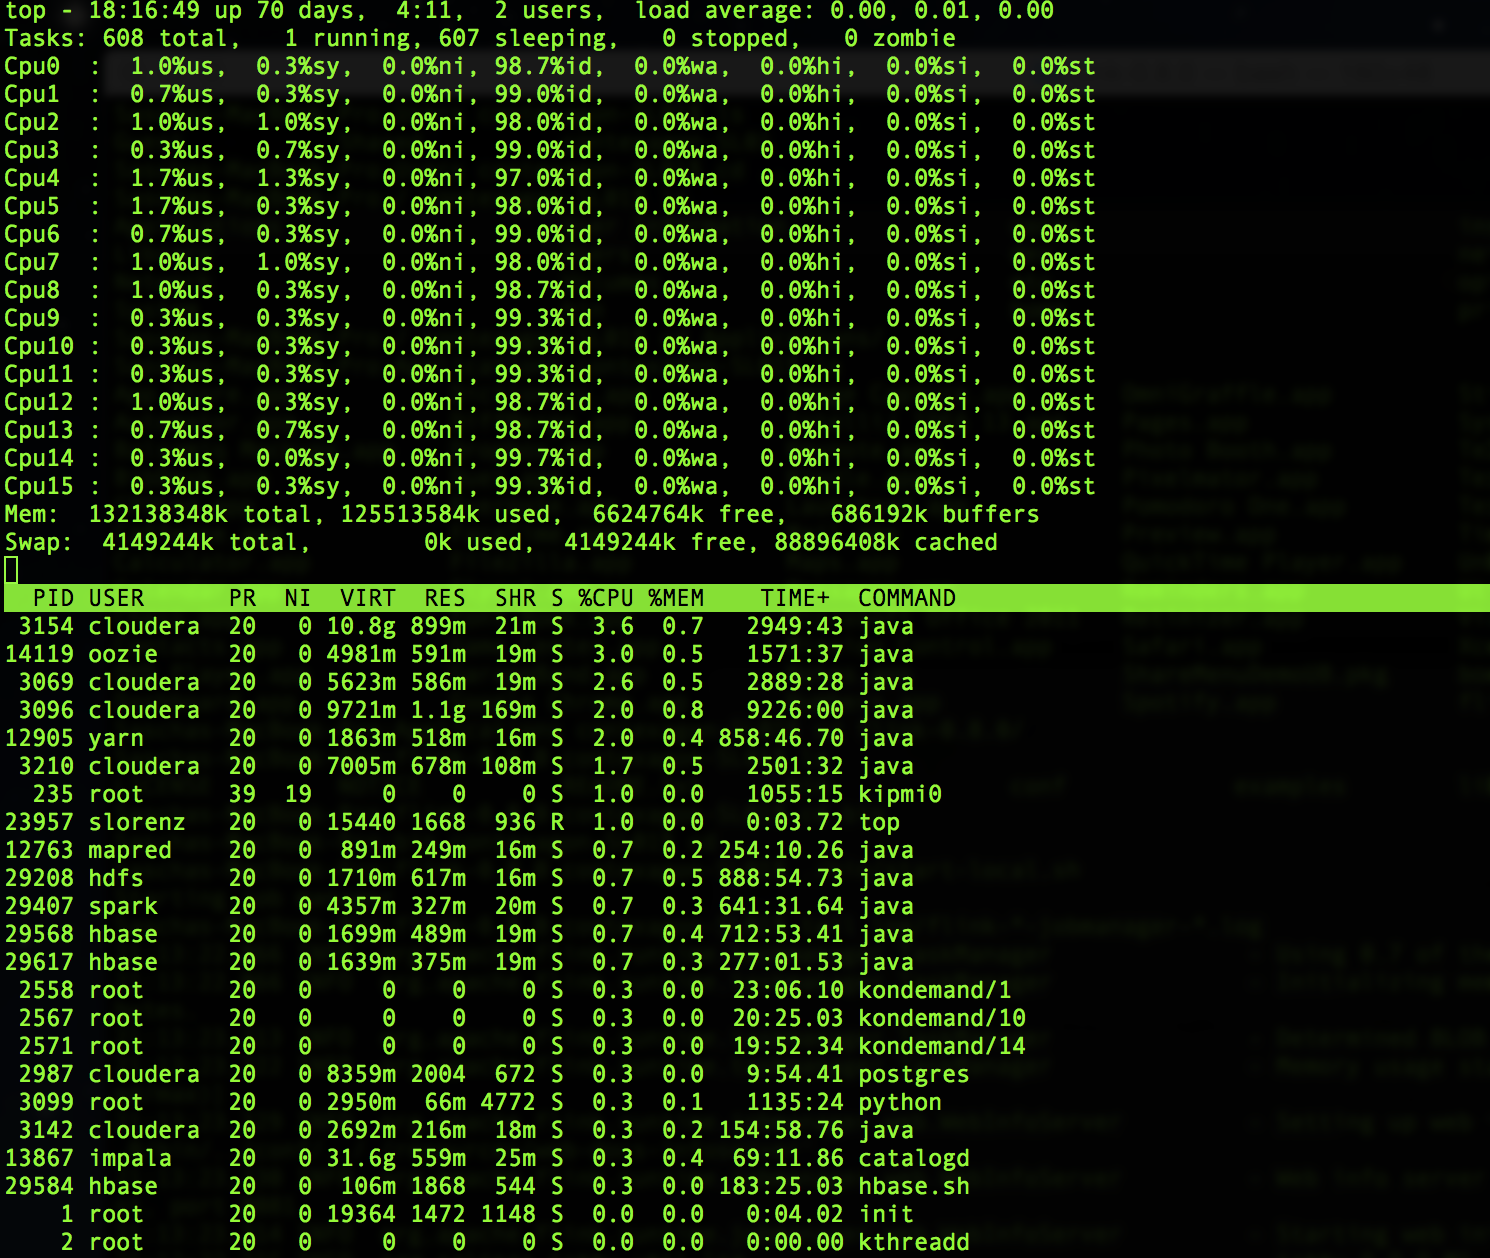
\includegraphics[width=1.0\textwidth]{bilder/top_cluster.png}
\caption{Ausführung des Linux-Befehls top auf dem Master-Node des Beuth-Clusters.}
\label{fig:topcluster}
\end{figure}    

Eine Einschränkung dieses Kommandos ist die fehlende Identifikation der benutzten Prozessorkerne bei Verwendung von Multicore-Systemen. Die prozentuale Prozessorauslastung wird pro Kern angegeben. Am Beispiel des unter anderem eingesetzten MacBook Pro mit i7 Prozessor (vier physische Kerne, acht mit Hyperthreading) bedeutet dies, dass eine Maximalauslastung der CPU bei dieser Metrik einen Wert von 800\% erreicht. Außerdem lässt sich bei einer dargestellten Auslastung von 100\% so nicht ermitteln, ob es sich bei diesem Wert um einen Thread mit 100\% Auslastung eines Kernes, um zwei Threads mit 80\% und 20\%, oder um vier unabhängige Threads mit je 25\% Kernauslastung handelt. Aus diesem Grund werden für die Metriken zusätzlich zu der prozentualen Angabe der CPU-Auslastung die CPU-Zeit als Messgrößen verwendet. Diese ist proportional zur Prozessorauslastung. Für die durchgeführten Vergleichsmessungen werden die CPU-Zeiten der Standardimplementierung des BDAS mit 100\% gewertet und die Vergleichsalgorithmen dazu in das entsprechende Verhältnis gesetzt.  

Da Spark die RDDs wenn möglich im Hauptspeicher hält und nur auf Festspeicher auslagert, wenn das RAM nicht ausreichend ist, wird auf ein Monitoring des Hauptspeichers für diese Messungen verzichtet. Statt dessen werden die I/O-Vorgänge überwacht um so einen Überlauf auf den Festspeicher und damit begründete Performance-Einbrüche feststellen zu können. 




\section{Beschreibung der Messumgebungen}
\label{section:messumgebungen}

Zum Einsatz für die Evaluierung kamen für diese Untersuchung unterschiedliche Ansätze für Clusterinfrastrukturen. Es kamen diverse lokale Installationen, sowie ein leistungsfähiges Rechnercluster an der Beuth Hochschule Berlin zum Einsatz.  

Die Tabelle \ref{tab:lokale hardware} gibt eine detaillierte Übersicht über die lokal verwendeten Hardwarekonfigurationen. Alle lokal eingesetzten Maschinen verfügen über SSDs (Solid State Drives) als Festspeicher.

\begin{table}[!ht]
\centering
\begin{tabular}{| p{3cm} | p{2.2cm} |  p{3cm} |  p{1.2cm} | p{3cm} | }
\hline
System & CPU & Anzahl Cores & RAM & OS\\ \hline \hline
MacBook Pro Mid 2014 & Intel i7 & 4 physisch, 8 mit Hyperthreading & 16 GB & Mac OS-X 10.10.2 Yosemite \\ \hline
Apple iMac Mid 2011 & Intel i5 & 4 physisch, 8 mit Hyperthreading & 16 GB & Mac OS-X 10.10.2 Yosemite \\ \hline
Xeon Workstation & Intel Xeon 1230 & 4 physisch, 8 mit Hyperthreading & 32 GB & Windows 8.1,  VirtualBox Instanzen mit CentOS  \\ \hline 
Lenovo ThinkPad 410T & Intel i5 & 4 physisch & 8 GB & Windows 8.1, VirtualBox Instanzen mit CentOS  \\ \hline 

\end{tabular}
\caption{Übersicht der lokal verwendeten Hardware}
	\label{tab:lokale hardware}
\end{table}  

Die Tabelle \ref{tab:cluster} zeigt die Konfiguration (Konfigurationsstand Dezember 2014) des verwendeten Clustersystems an der Beuth Hochschule Berlin. 

\begin{table}[!ht]
\centering
\begin{tabular}{| p{3cm} | p{2.2cm} |  p{3cm} |  p{1.2cm} | p{3cm} | }
\hline
System & CPU & Anzahl Cores & RAM & OS\\ \hline \hline
Master Node & AMD 6320 & 2 * 8  & 128 GB & Debian Linux \\ \hline
Worker Node 1 & AMD 6378 & 4 * 16 & 512 GB &  Debian Linux\\ \hline
Worker Node 2 & AMD 6378 & 4 * 16 & 512 GB &  Debian Linux\\ \hline
Worker Node 3 & AMD 6378 & 4 * 16 & 512 GB &  Debian Linux\\ \hline

\end{tabular}
\caption{Übersicht über das Cluster der Beuth Hochschule Berlin}
	\label{tab:cluster}
\end{table}  


\newpage

\subsection{Lokales Single Node Cluster  }
\label{section:lokales single node}

TBD!

\subsection{Lokales Multi Node Cluster}
\label{section:tachyon}

TBD!

\subsection{Remote Cluster an der Beuth Hochschule}
\label{section:remote}

TBD!

\section{Ergebnisse}
\label{section:ergebnisse}

TBD!

\subsection{Messergebnisse Apache Spark}
\label{section:spark eval}

Apache Spark wurde mit den zwei im Kapitel \ref{chapter:implementierung} beschriebenen Prototypen gemessen. Die Messungen wurden gegen verschiedene Metriken durchgeführt. In Diagramm \ref{fig:cpu4th} wird exemplarisch eine solche Messung gezeigt. Hier wurde der Prototyp SimpleSparkPrototype, der das Vorkommen zweier verschiedener Buchstaben in einem unstrukturierten Text zur Aufgabe hat, gemessen. Es wurden Testdaten mit einer Größe von ca. 3,5 GB verwendet, die aus einem Subset der Zugriffslogs von Wikipedia bestehen. 

Das Diagramm zeigt den Verlauf der CPU-Auslastung mit vier zugewiesenen Threads. Wie zu erkennen ist, werden die ersten rund 17 Sekunden der Gesamtlaufzeit von 46 Sekunden für die Initialisierung und den Start von Spark benötigt. Dies nimmt verhältnismäßig viel Zeit in Anspruch, da hier sowohl der Spark-Context für die Verwaltung des Clusters, als auch der Webserver für die Überwachung des Spark-Clusters initialisiert werden. Die folgenden Messungen zeigen diese Ramp-Up-Phase von Spark nicht mehr, sondern starten erst mit dem Lesen der Quelldaten und dem Transformationsschritt.  

\begin{figure}[htb!]
\centering
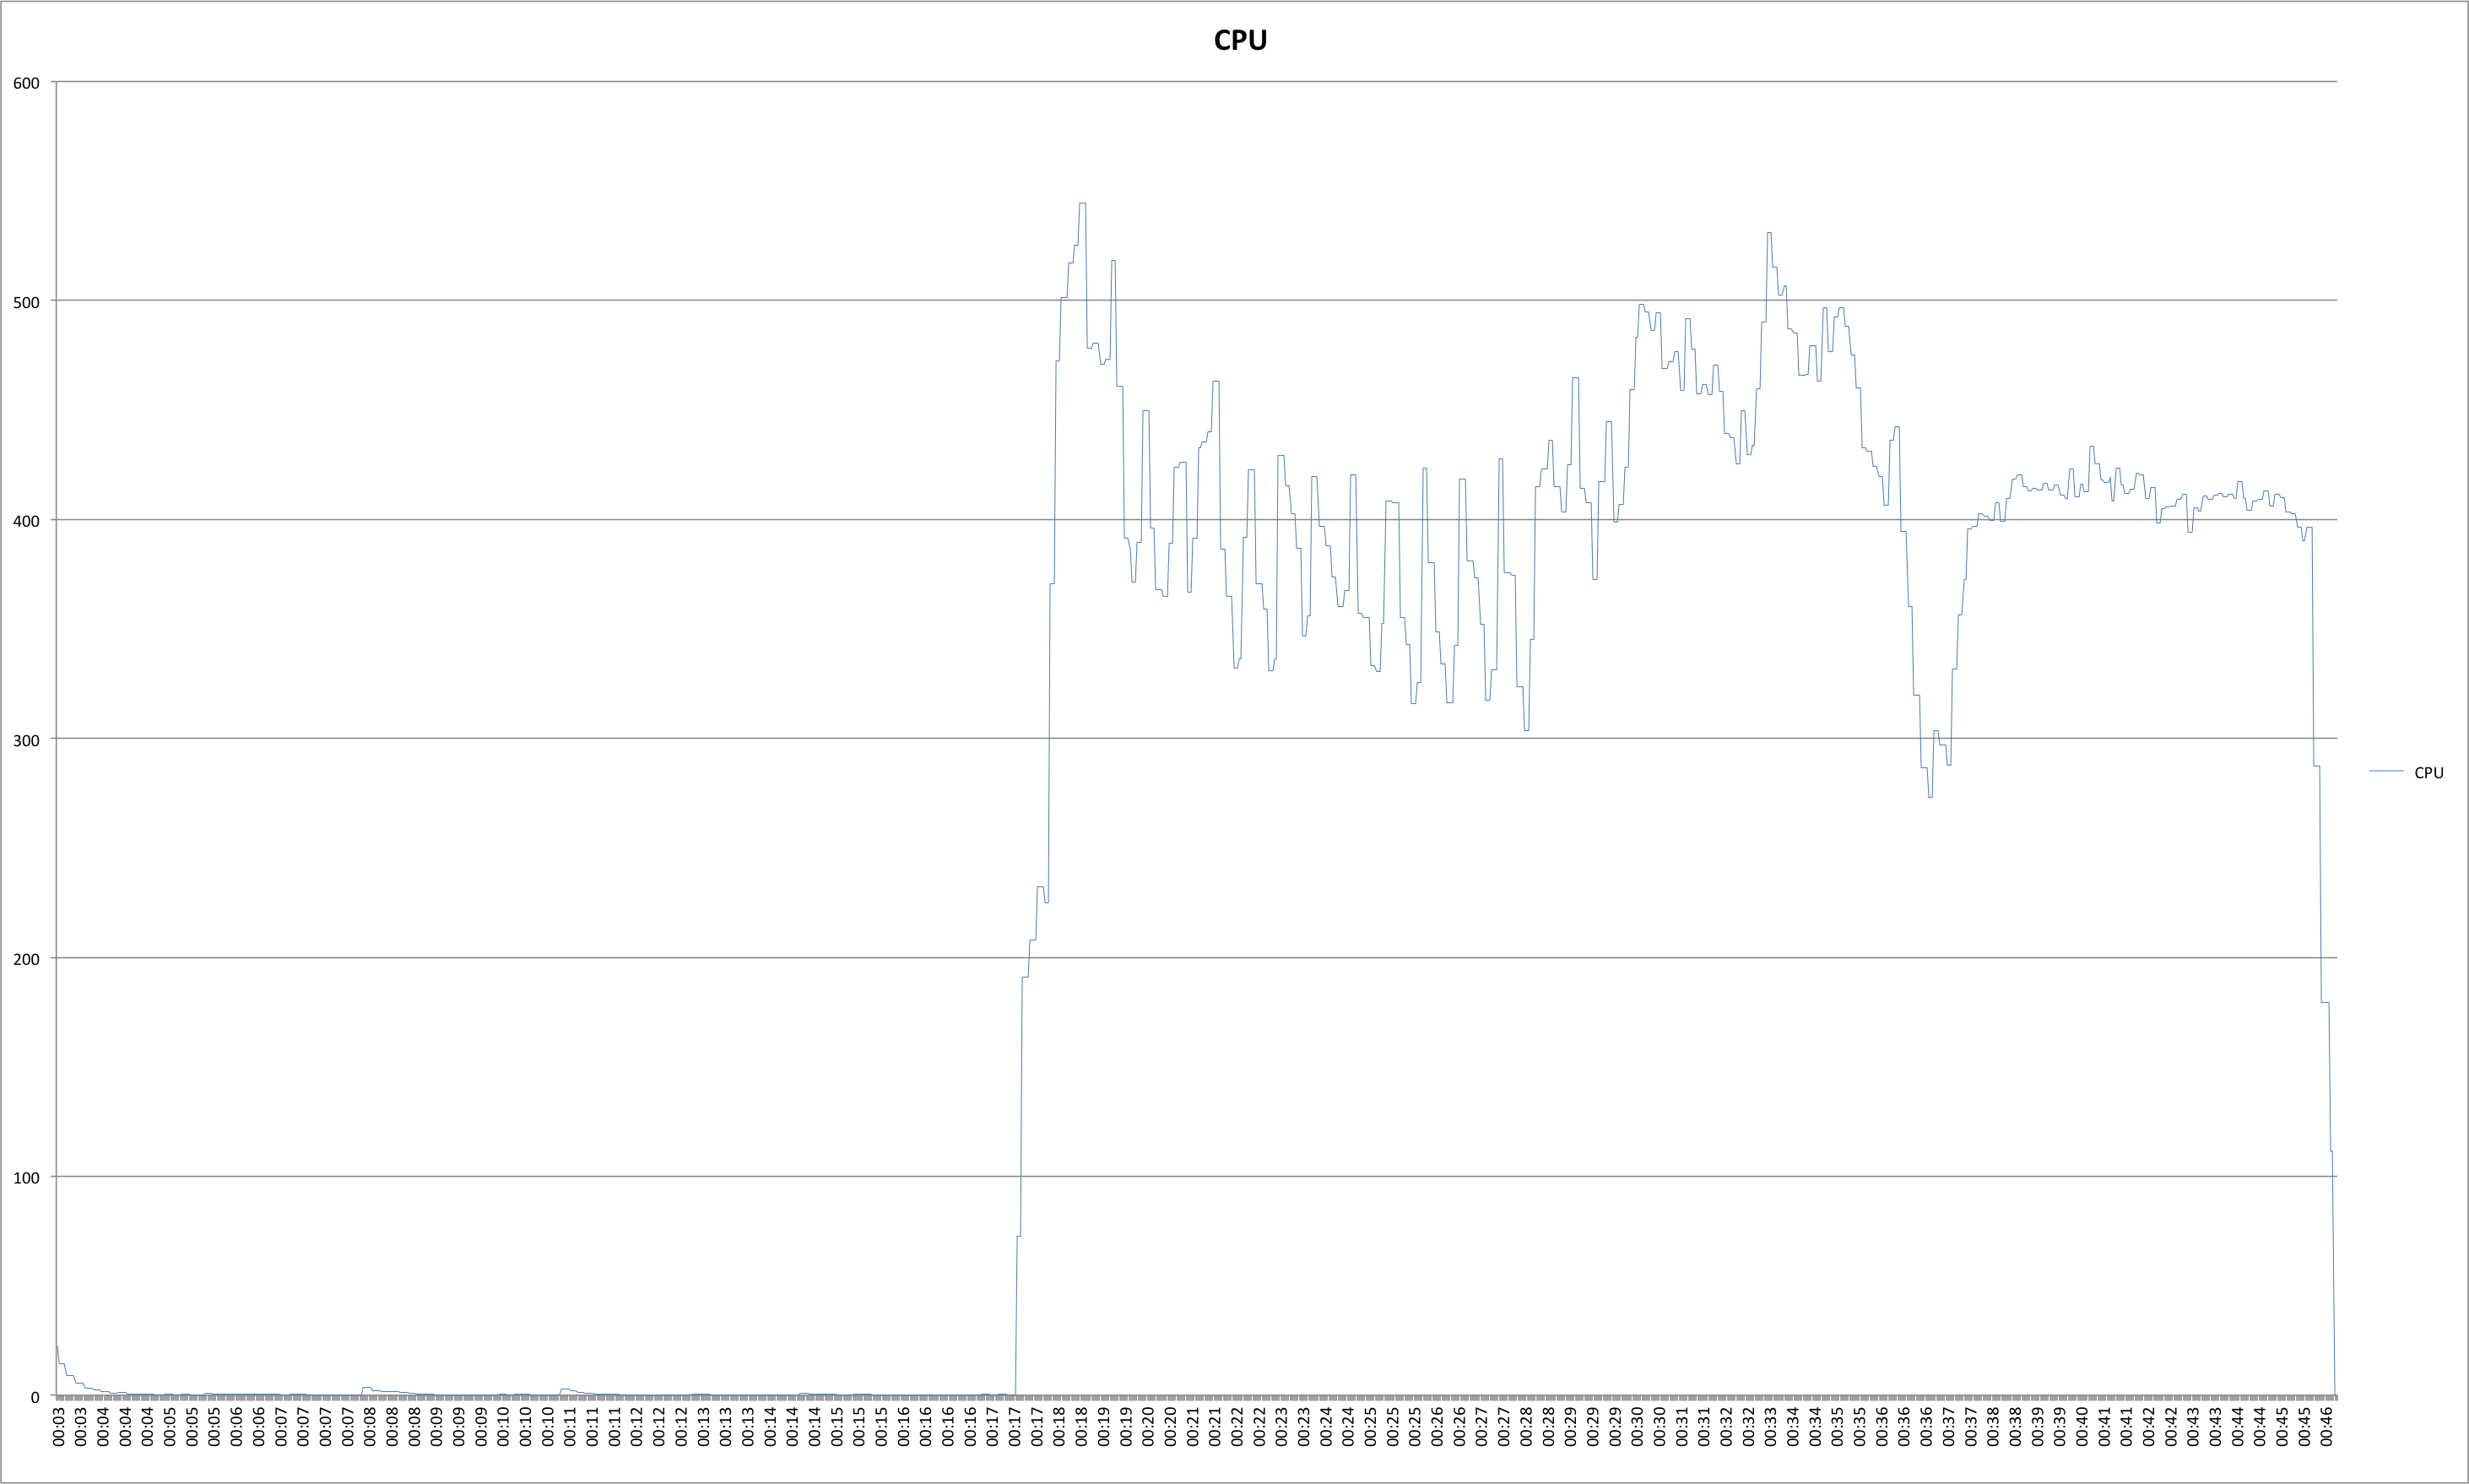
\includegraphics[width=1.0\textwidth]{bilder/SparkCharCount4Thr.png}
\caption{Messung der Laufzeit und CPU-Auslastung des CharCounters mit 4 Threads}
\label{fig:cpu4th}
\end{figure}   

\subsection{Messergebnisse Apache Flink}
\label{section:mllib arch}

TBD!

\subsection{Messergebnisse MLLib}
\label{section:mllib arch}

TBD!

\subsection{Messergebnisse H2O}
\label{section:mllib arch}

TBD!



\section{Zusammenfassung}
\label{section:zusammen}



TBD!

\chapter{Schlussbetrachtung }
\label{chapter:schlussbetrachtung}


Blablabla 


\section{Zusammenfassung}
\label{section:zusammenfassung}

Blablba

\section{Ausblick}
\label{section:ausblick}





%%%%%%%%%%%%%%%%%%%%%%%%%%%%%%%%%%%%%%%%%%%%%%%%%%%%%%%%%%%%%%%
%% Verzeichnisse

\chapter{Verzeichnisse}
\label{chapter:verzeichnisse}
%\addcontentsline{toc}{chapter}{Verzeichnisse}

\bibliographystylelit{geralpha}
\bibliographylit{literaturVerzeichnis}
\addcontentsline{toc}{section}{Literaturverzeichnis}

%\newpage
\bibliographystyleint{geralpha}
\bibliographyint{internetQuellen}
\addcontentsline{toc}{section}{Internetquellen}

%\newpage
\listoffigures
\addcontentsline{toc}{section}{Abbildungsverzeichnis}
\clearpage
\cleardoublepage
%\newpage
\listoftables
\addcontentsline{toc}{section}{Tabellenverzeichnis}
\clearpage
\cleardoublepage
\lstlistoflistings 
\addcontentsline{toc}{section}{Quellenverzeichnis}
\clearpage
\cleardoublepage

%%%%%%%%%%%%%%%%%%%%%%%%%%%%%%%%%%%%%%%%%%%%%%%%%%%%%%%%%%%%%%%
%% Anhang

\clearpage\newpage
\begin{appendix}
  %%
%% Beuth Hochschule für Technik --  Abschlussarbeit
%%
%% Anhang
%%
%%%%%%%%%%%%%%%%%%%%%%%%%%%%%%%%%%%%%%%%%%%%%%%%%%%%%%%%%%%%%%%%%%%%%

\chapter{Zusätze}
\label{chapter:anhang}

\setglossarysection{section}
\printglossary[type=\acronymtype,title=Abkürzungen]


\section{Quelltext}
\label{section:quelltext}



\end{appendix}



\end{document}
